%\documentclass[a4paper, 10 pt, conference]{ieeeconf_ilker}
%\IEEEoverridecommandlockouts
%\overrideIEEEmargins

\documentclass[letterpaper, 10 pt, conference]{ieeetran}  % Comment this line out if you need a4paper
                                                   
%\documentclass[a4paper, 10pt, conference]{ieeeconf}      % Use this line for a4 paper

\IEEEoverridecommandlockouts                              % This command is only needed if 
                                                          % you want to use the \thanks command

\overrideIEEEmargins                                      % Needed to meet printer requirements.
                                                          % you want to use the \thanks command
                                                          
% \overrideIEEEmargins                                      % Needed to meet printer requirements.
\pdfminorversion=4 

% setup page to suit conference specification using fancyhdr
%\usepackage{fancyhdr}
%\setlength{\paperwidth}{215.9mm}
%\setlength{\hoffset}{-9.7mm}
%\setlength{\oddsidemargin}{0mm}
%\setlength{\textwidth}{184.3mm}
%\setlength{\columnsep}{6.3mm}
%\setlength{\marginparsep}{0mm}
%\setlength{\marginparwidth}{0mm}

%\setlength{\paperheight}{279.4mm}
%\setlength{\voffset}{-7.4mm}
%\setlength{\topmargin}{19mm}
%\setlength{\headheight}{0mm}
%\setlength{\headsep}{0mm}
%\setlength{\topskip}{0mm}
%\setlength{\textheight}{235.2mm}
%\setlength{\footskip}{12.4mm}

%\setlength{\parindent}{1pc}


% correct bad hyphenation here
\hyphenation{op-tical net-works semi-conduc-tor}
\usepackage{blindtext}
\usepackage{tikz}
\usepackage[utf8]{inputenc}
\usepackage[english]{babel}
\usepackage{subcaption}  % Add this in the preamble if not already included

\usepackage[ruled,vlined,linesnumbered]{algorithm2e}
\usetikzlibrary{positioning}
\usetikzlibrary{shapes.geometric}
\usetikzlibrary{arrows.meta}
\usepackage{subfig}
\usepackage[nolist]{acronym}
\usepackage[table, dvipsnames]{xcolor}
\usepackage[pdftex]{graphicx} % graphics package
\usepackage{graphicx}
\usepackage[colorinlistoftodos]{todonotes}
%\usepackage[lofdepth,lotdepth,caption=false]{subfig} % subplot package
\usepackage{graphicx}
\usepackage{caption}
\usepackage{algorithm}
\usepackage{algpseudocode}
\captionsetup{compatibility=false}
\usepackage{subcaption}
\usepackage{tikz}
\usetikzlibrary{shapes.geometric, arrows}
\usepackage{array} % for defining custom column types
\usepackage{amssymb} %we added the package to the document
\usepackage{algorithm}
\usepackage{algpseudocode}
\usepackage{amsmath}  %

\usepackage{algorithm}
\usepackage{algorithmicx}
\usepackage{algpseudocode}
\usepackage{amsmath}
\usepackage[small]{caption} % Reduce text size

\usepackage{booktabs}
\graphicspath{{figures/}} % declare the path where graphic files are
\DeclareGraphicsExtensions{.pdf,.jpg,.png} % grafic files extensions
\usepackage{amsmath} % math package for split
\usepackage{amsfonts} % math package for fonts
\usepackage{mathtools} % math package for tools like prescript
\usepackage{tikz} % figure package
\usetikzlibrary{shapes,arrows,fit,calc,positioning,automata,backgrounds}
%\usepackage{dblfloatfix} % figure package for positioning figures on the bottom
\usepackage{color} % colors package
\usepackage{multirow} % multiple rows in table
\usepackage{hhline} % separator in 
\usepackage{booktabs}
\usepackage[bookmarks=false, breaklinks]{hyperref} % hyperlink package
\usepackage{enumerate} % enumerate package
\usepackage{epstopdf} % package to include eps. files
\usepackage{dsfont}
\usepackage{siunitx} % package for international system units
\usepackage{cite}   % for compact citations, i.e. [1, 2]
\usepackage{diagbox}    % for making slash cell in a table
\usepackage{pdfpages}   
\usepackage{breqn}
\usepackage{svg}
\usepackage{multicol}
\svgpath{{images/svg/}} % <- using \svgpath to avoid warning
\colorlet{Green1}{green!90!}
\colorlet{Green2}{green!60!}
\colorlet{Green3}{green!40!}
\colorlet{Green4}{green!20!}
\colorlet{Green5}{green!10!}

% Used in order to break URL into smaller sections when seeing / or -
\usepackage{url}
\def\UrlBreaks{\do\/\do-}
\usepackage{breakurl}

%% ORCID
\RequirePackage{tikz} % For \foreach used for Orcid icon
% Make Orcid icon
\newcommand{\orcidicon}{\includegraphics[width=0.32cm]{images/orcid/logo-orcid.eps}}

% Define link and button for each author
\foreach \x in {A, ..., Z}{%
\expandafter\xdef\csname orcid\x\endcsname{\noexpand\href{https://orcid.org/\csname orcidauthor\x\endcsname}{\noexpand\orcidicon}}
}

\newcommand{\orcidauthorA}{0000-0001-5387-7613} % Add \orcidA{} behind the author's Hakim
\newcommand{\orcidauthorB}{0000-0003-3581-9481} % Add \orcidB{} behind the author's Olaya
\newcommand{\orcidauthorC}{0000-0002-1609-5783} % Add \orcidC{} behind the author's name  Halil
\newcommand{\orcidauthorD}{0000-0002-7742-6996} % Add \orcidD{} behind the author's name  Jonas
\newcommand{\orcidauthorE}{0009-0002-0445-8126} % Add \orcidE{} behind the author's name  Yury
\newcommand{\orcidauthorF}{0000-0002-7143-8777} % Add \orcidF{} behind the author's name  Erdal


% TikZ style definitions
\tikzstyle{startstop} = [rectangle, rounded corners, minimum width=3cm, minimum height=1cm, text centered, draw=black, fill=blue!20]
\tikzstyle{process} = [rectangle, minimum width=3cm, minimum height=1cm, text centered, draw=black, fill=green!20]
\tikzstyle{decision} = [diamond, minimum width=3cm, minimum height=1cm, text centered, draw=black, fill=red!20]
\tikzstyle{arrow} = [thick,-{Latex[length=3mm, width=2mm]}]



\definecolor{Bookcolor}{HTML}{00F9DE}
\definecolor{darkgreen}{rgb}{0.0, 0.5, 0.0}
\definecolor{gray}{gray}{0.9}
\definecolor{lightgray}{rgb}{0.86, 0.86, 0.86}

\makeatletter
\def\@citex[#1]#2{\leavevmode
\let\@citea\@empty
\@cite{\@for\@citeb:=#2\do
{\@citea\def\@citea{,\penalty\@m\ }%
\edef\@citeb{\expandafter\@firstofone\@citeb\@empty}%
\if@filesw\immediate\write\@auxout{\string\citation{\@citeb}}\fi
\@ifundefined{b@\@citeb}{\hbox{\reset@font\bfseries ?}%
\G@refundefinedtrue
\@latex@warning
{Citation `\@citeb' on page \thepage \space undefined}}%
{\@cite@ofmt{\csname b@\@citeb\endcsname}}}}{#1}}
\makeatother


\newcommand{\HP}[1]{\textcolor{blue}{[HP: #1]}}
\newcommand{\HIU}[1]{\textcolor{red}{[HIU: #1]}}
\newcommand{\KA}[1]{\textcolor{orange}{[KA: #1]}}
\newcommand{\EK}[1]{\textcolor{magenta}{[EK: #1]}}
\newcommand{\JFS}[1]{\textcolor{darkgreen}{[JFS: #1]}}
\newcommand{\note}[1]{\textcolor{red}{[NOTE: #1]}}

\DeclareMathOperator*{\minimize}{{min}}
\DeclareMathOperator*{\maximize}{{max}}

\newcommand{\bm}[1]{\mathbf{#1}}

\begin{acronym}
    % \acro{CAMAP}{conflict-aware multi-agent planner}
{
    \acro{MPC}{model predictive control}
    \acro{GP}{Gaussian process}
    \acro{AUV}{autonomous underwater vehicle}
    \acro{MHE}{moving horizon estimator}
    \acro{EKF}{extended kalman filter}
    \acro{ROV}{remotely operated vehicle}
    \acro{TSP}{traveling salesman problem}
    \acro{IMU}{inertial measurement unit}
    \acro{DVL}{doppler velocity log}
    \acro{NED}{North East Down}
    \acro{RTI}{real-time iteration}
    \acro{OCP}{optimal control problem}
    \acro{LP}{linear program}
    \acro{MIP}{mixed integer program}
    \acro{EA-MPC}{entanglement aware model predictive control}
    \acro{TSDF}{ truncated signed distance field}
    \acro{SDF}{ signed distance field}
    \acro{CPP}{ coverage path planner}
    \acro{OEA-PP}{online entanglement aware path planner}
    \acro{OMPL}{open motion planning}
        \acroplural{ROV}[ROVs]{remotely operated vehicles}

\acro{REACT}{Real-time Entanglement-Aware Coverage Path Planning for Tethered Underwater Vehicles}

  % Ensures ROVs is treated the same as ROV
}


\end{acronym}




\begin{document}

%
%\title{Online Entanglement-Aware Path Planning for Safe Autonomous Underwater Vehicle Inspection}
\title{REACT: Real-time Entanglement-Aware Coverage Path Planning for Tethered Underwater Vehicles}

% author names and affiliations
% use a multiple column layout for up to three different affiliations
\author{Abdelhakim Amer, Mohit Mehindratta, Yury Brodskiy and Erdal Kayacan
%\author{
% <-this % stops a space
\thanks{A. Amer is with the Artificial Intelligence in Robotics Laboratory (AiR Lab), Department of Electrical and Computer Engineering, Aarhus University, 8000 Aarhus C, Denmark {\tt\small \{abdelhakim\} at ece.au.dk}.    Mohit Mehndiratta is with GIM Robotics, Espoo, Finland, {\tt\small \{mohit.mehndiratta\} at gimrobotics.fi}.
     Y. Brodskiy is with EIVA a/s, 8660 Skanderborg, Denmark. {\tt\small \{ybr\} at eiva.com.}
    E. Kayacan is with the Automatic Control Group, Department of Electrical Engineering and Information Technology, Paderborn University, Paderborn, Germany. {\tt\small \{erdal.kayacan\} at uni-paderborn.de}.}%
}

\maketitle
\begin{abstract}

Inspection of complex underwater structures with tethered underwater vehicles is often hindered by the risk of tether entanglement. We propose REACT (Real-time Entanglement-Aware Coverage Path Planning for Tethered Underwater Vehicles), a framework designed to overcome this limitation. REACT comprises a fast, geometry-based tether model using the signed distance field (SDF) map for accurate, real-time simulation of taut tether configurations around arbitrary structures. This model enables an efficient online replanning strategy within REACT that enforces a maximum tether length constraint, actively preventing entanglement. By integrating REACT into a coverage path planning framework, we achieve safe and optimal inspection paths, previously challenging due to tether constraints. To ensure safe and precise path following, a model predictive controller (MPC) is employed, accounting for system dynamics, while optimally following a desired trajectory. The complete REACT framework's efficacy is validated in a pipe inspection scenario, demonstrating safe, entanglement-free navigation and full coverage inspection.




% What is the problem this paper is trying to solve?

% What is the approach?


% What does the results show?

%
\end{abstract}

\begin{IEEEkeywords}
coverage path planning, autonomous underwater vehicle (AUV), model predictive control, signed distance field (SDF), tether modelling, tether constraints.
\end{IEEEkeywords}

\IEEEpeerreviewmaketitle

%\bstctlcite{IEEEexample:BSTcontrol}

% introduction and related work




\section{Introduction}
\label{sec:introduction}

% % Underwater Robot Applications:
%
%Operating in complex, hazardous, and otherwise inaccessible environments, \Acfp{ROV} have become essential for a diverse range of demanding applications, including surveying, infrastructure inspection, and search-and-rescue, significantly expanding operational possibilities~\cite{amer2023unav, amer2025modelling}.
%
% Why We Need Tether:
%
%Most \acp{ROV} are tethered to ensure a continuous power supply during long-duration missions and to maintain reliable communication.

Operating in complex, hazardous, and otherwise inaccessible environments has made \acp{ROV} essential tools in modern exploration and intervention tasks. They facilitate a diverse range of demanding applications, including surveying, infrastructure inspection, and search and rescue missions, thus significantly expanding operational possibilities \cite{amer2023unav, amer2025modelling}. Most \acp{ROV} are tethered to a host platform to maintain reliable communication and ensure a continuous power supply during long-duration missions. However, this tethering infrastructure introduces operational challenges related to planning and control while posing the risk of being entangled with underwater objects such as flora, fauna, or structures under inspection.

%
% Introducing Problem Definition:
%
%However, the presence of a tether introduces complexities in path planning and control, as it poses a risk of entanglement with underwater objects such as flora, fauna, or the underwater structures being inspected.

%Tether-related challenges restrict the applicability of path-planning algorithms originally designed for untethered systems. For instance, numerous \ac{CPP} algorithms exist to compute distance-optimal paths for covering 3D structures \cite{bircher2015structural,feng2024fc, amer2023visual}. Additionally, exploration path planners are employed to determine the next viewpoints for mapping and exploring unknown terrains \cite{dang2020graph}. However, these methods do not account for entanglement with the surroundings and thus cannot be directly applied to tethered underwater robots.

Numerous \ac{CPP} algorithms are proposed in the literature for inspection-related tasks with untethered systems. In essence, they compute distance-optimal paths for a thorough inspection of 3D structures \cite{bircher2015structural,feng2024fc, amer2023visual}.  Additionally, exploration path planners are employed to determine the next viewpoints for mapping unknown terrains \cite{dang2020graph}. However, these path-planning methods are restricted to untethered systems, as they do not account for possible entanglements with the surroundings. Hence, the literature still lacks path-planning algorithms that directly address tether-related challenges.

%
% Entanglement Problem and Definition:
%
In case of underwater inspection, entanglement occurs when the vehicle's movement is restricted due to interaction between the tether and objects in the environment. The tether can loop around obstacles, thereby limiting the vehicle's mobility and substantially reducing operational range in a worst-case scenario. Consequently, operators need to carry longer tethers to account for possible entanglements without a proper planner at hand.
In this work, we propose the \ac{REACT} algorithm that fills this critical gap in underwater asset inspection. In essence, when integrated into the coverage path planning framework, \ac{REACT} renders entanglement-free paths, thus ensuring task completion without the need to carry additional tether lengths. Besides, the proposed planning framework reduces overall operational time by circumventing the post-completion detangling process, often required with traditional path-planning methods. The contributions of this work can be summarized as follows:
\begin{itemize}
\item A computationally efficient tether model that computes the tether configuration in real-time using \ac{SDF} data of arbitrary underwater structures.
\item An efficient online replanning method that prevents entanglement by incorporating a tether-length constraint.

\item Integration with an off-the-shelf \ac{CPP} along with \ac{MPC}, rendering optimal trajectory following.
\item Demonstration of the framework in simulation and real-world tests, showcasing its ability to ensure safe and time-efficient inspection.
\end{itemize}


%
\begin{figure}[t!]
	\centering	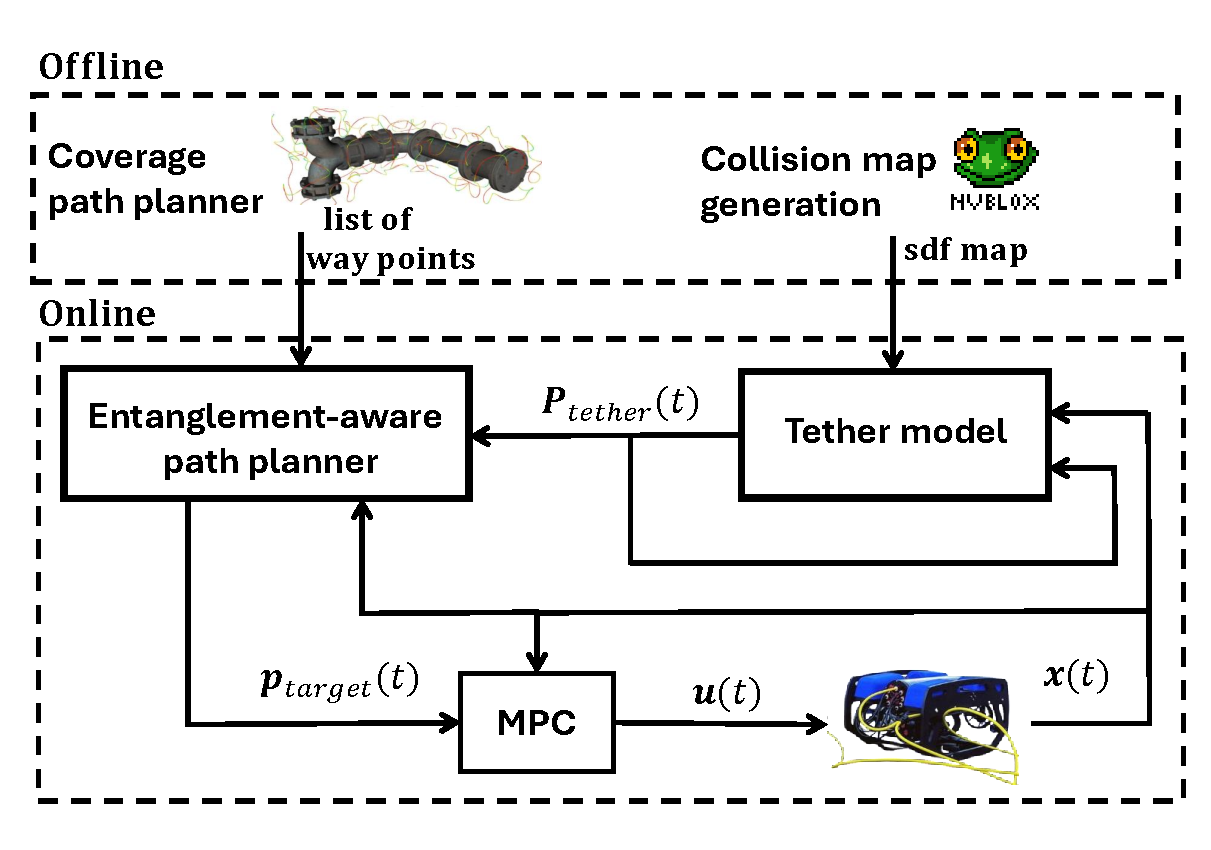
\includegraphics[width=1\linewidth]{EA-Planner/figures/abstract.pdf}
	  \caption{\textcolor{black}{Overview of the \ac{REACT} inspection framework. Offline, a \ac{SDF} map is generated from a point cloud, and an off-the-shelf \ac{CPP} \cite{feng2024fc} is used to compute an optimal waypoint sequence. During operation, a tether model $(\mathbf{P}_{tether}(t))$ is used  to ensure tether length is not exceeded, while an \ac{MPC} controller applies the optimal wrench $\mathbf{u}(t)$ to the \ac{ROV}}.}
    \label{fig:abstract}
\end{figure}
%







The remainder of this paper is organized as follows: Section \ref{sec:related_work} reviews the state of the art. Section \ref{sec:framework} presents the path planning framework for underwater structure inspection with tether constraints. Section \ref{sec:tether_model} introduces the taut-tether model, and Section \ref{sec:planner} details the online entanglement-aware path planner. Experimental results are presented in Sections \ref{sec:simulationexperiments} and \ref{sec:real-world}, followed by conclusions in Section \ref{sec:conclusion}.





 
\section{State of the art}
\label{sec:related_work}

% Paragraph 1: Introduction to Tether Importance and Entanglement Definition
Tethers play a vital role in numerous mobile robotics applications, offering crucial power delivery and reliable data transmission. However, the risk of entanglement with obstacles presents a significant planning challenge. To systematically address this, a taxonomy of entanglement definitions has been presented in \cite{definitions}, cataloging existing interpretations from the literature and introducing new definitions, paving the way for developing new path planning strategies that account for entanglement.

% Paragraph 2: Early Approaches - 2D Offline Path Planning (Single Robot)
Initial efforts to develop entaglement-aware path planners often focused on two-dimensional environments and employed offline computation strategies. For instance, \cite{rov_mccammon} and \cite{mechsy2017novel} proposed methods for planning paths in 2D to cover a predefined set of waypoints while considering tether constraints. Notably, \cite{mechsy2017novel} formulated the path planning problem for a \ac{ROV} as a mixed-integer programming problem. Their approach first solves a \ac{TSP} to find an optimal waypoint sequence and then incorporates homotopic constraints during path generation to minimize the likelihood of tether entanglement. While effective for predefined scenarios, these offline methods lack the adaptability required for dynamic environments. A more recent approach \cite{peng2025spanning} tackles the 2D coverage path planning problem for tethered robots using spanning tree-based offline optimization.

% Paragraph 3: Advancements - 2D Online Path Planning (Single Robot)
Addressing the need for real-time adaptability, subsequent research explored online path planning algorithms, still primarily in 2D. \cite{kim} introduced a homotopy-augmented topological approach combined with graph search techniques, allowing for dynamic adjustments to the path based on environmental perception. Similarly, \cite{withy} developed a hybrid A* variant that utilizes a modified tangent graph. This method efficiently plans curvature-constrained paths for tethered robots subject to winding angle constraints, demonstrating guarantees and providing simulation results for online entanglement avoidance. 

% Paragraph 4: Scaling Complexity - Multi-Robot Systems in 2D
The complexity of tether management increases significantly when coordinating multiple robots. Several approaches have tackled this challenge in 2D. Early work by \cite{hert1996ties} laid groundwork in this area, followed by methods like \cite{zhang2019planning}. More recently, \cite{cao2023neptune} presented an efficient online path planner for multi-robot systems. Their method integrates a homotopy-based high-level planner with trajectory optimization and smoothing techniques to generate entanglement-free paths. However, despite its online capability, this approach remains constrained to 2D environments. 

The above presented online planners represent a significant step towards real-time tether management; however, they are limited to 2D environments. Moreover, while they can plan preventive paths to avoid entanglement, they do not provide a strategy for path planning once tether entanglement has already occurred.

% Paragraph 5: Moving to Three Dimensions - 3D Path Planning (Single Robot)
Real-world applications frequently require navigation in 3D environments, such as with underwater robots. Consequently, work by  \cite{bhattacharya2012topological} and \cite{martinez2021optimization} explored topological aspects and optimization techniques for 3D tethered navigation. \cite{petit2022tape} specifically presented a 3D exploration path planner that incorporates explicit contact avoidance constraints for the tether, facilitating safer navigation for single tethered robots in complex three-dimensional spaces.

% Paragraph 6: 3D Multi-Robot Path Planning
 \cite{hert1999motion} extended their earlier 2D work to handle the increased complexity of 3D multi-robot scenarios. Further advancements by \cite{patil2023coordinating} and  \cite{cao2023path} introduced path planning strategies that explicitly consider the topological constraints imposed by multiple interacting tethers in 3D. While these methods advance the state-of-the-art in multi-robot coordination, they are generally designed for offline computation and are not suited for online path planning where real-time implementation is essential.

% Paragraph 7: Identifying the Research Gap
% Summarize the limitations of existing work: 
In summary, existing path planners that accounts for tether constraints often face limitations for practical online \ac{CPP} in complex 3D settings. Many are too computationally intensive for real-time use \cite{mechsy2017novel, hert1999motion, patil2023coordinating, cao2023path}, lack integrated tether-aware CPP frameworks, or rely on simplifying assumptions like 2D environments or basic obstacle shapes \cite{kim, withy, cao2023neptune}, hindering generalization to real-world inspection tasks.
% Paragraph 8: Introducing the Proposed Solution (REACT) based on its key contributions
To address these limitations, we propose \ac{REACT}, a novel approach that enables real-time, entanglement-aware path planning in arbitrary 3-D environments.


% --- End of Literature Review Section ---













































% % Introduce tether in literature
% Tether considerations in autonomous robot planning has drawn increasingly attention in robotics literature due to their critical role in enabling robots to operate autonomously in unknown environments for a wide range of mobile robots. 
% % Entaglement definitions
% A taxonomy of entanglement definitions is presented in \cite{definitions} which catalogs existing definitions from the literature and also introduces six new definitions.  These definitions open the door to the design of new entanglement aware path planning approaches.

% % 2-D , offline
% Regarding the path planners, many path planning methods have been proposed to address tether entanglement in 2-D environments. \cite{rov_mccammon} and \cite{mechsy2017novel} propose 2-D offline path planning to cover a set a way-points. In particular, \cite{mechsy2017novel} formulate the path planning problem for a \ac{ROV} as a mixed-integer programming problem. Their method solves a \ac{TSP} to determine the optimal sequence of waypoint visits, while incorporating homotopic constraints to reduce the likelihood of tether entanglement.
% % 2-D , online
% Also in 2-D, but in an online fashion, a homotopy-augmented topological approach, combined with graph search techniques is proposed by \cite{kim}. In addition to offline methods, online path planners allow real-time entanglement avoidance \cite{kim}, \cite{withy}. A hybrid A* variant uses a modified tangent graph to efficiently plan curvature-constrained, tethered robot paths under winding angle constraints, with guarantees and simulation results provided \cite{withy}.
% % 2-D , Multirobot
% Other approaches, also in 2-D address the tether constraints problem for the multi-robot case in \cite{zhang2019planning}, \cite{hert1996ties}, and \cite{cao2023neptune}. An efficient online path planner is presented in \cite{cao2023neptune}, combining a homotopy-based high-level planner with trajectory optimization and smoothing to generate entanglement-free paths for multi-robot systems. However, this approach is limited to 2-D environments. 
% % 3-D , Multirobot
% Entanglement avoidance has also been investigated in 3-D environments, as demonstrated in \cite{petit2022tape}, \cite{martinez2021optimization}, and \cite{bhattacharya2012topological}. In particular, \cite{petit2022tape} presents a 3-D exploration path planner that incorporates contact avoidance constraints on the tether, enabling safe navigation for tethered robots in three-dimensional spaces. For multi-robot operations, \cite{hert1999motion} extends earlier work to handle the increased complexity of coordinating multiple tethered robots. Further advancements by \cite{patil2023coordinating} and \cite{cao2023path} introduce improved coordination strategies that consider topological constraints imposed by multiple tethers. However, these approaches are not designed for real-time, online path planning.

% % NICHE and summary of research gap 
% In summary, most existing planners suffer from limitations that hinder their use in practical, online coverage path planning applications. Many are too computationally intensive for real-time implementation, and there is a lack of coverage path planning frameworks that explicitly account for the tether during planning. Existing tether-aware methods often rely on simplifying assumptions, such as 2-D environments or simplistic obstacle shapes (e.g., circles or cylinders), and thus fail to generalize to complex, real-world environments—particularly in inspection tasks.
% % Introduce REACT
% To address these limitations, we propose \ac{REACT}, a novel approach that enables real-time, entanglement-aware path planning in arbitrary 3-D environments.

 
\section{Overall \ac{REACT}  Framework}
\label{sec:framework}
\ac{REACT} framework, as depicted in \ref{fig:abstract}, consists of two main components: an offline planning phase and an online execution phase. In the offline phase, the environment is provided as a point cloud, including the object to be inspected. Then, a \ac{SDF} map is generated from this point cloud using the nvblox library \cite{nvblox}. Subsequently, the extracted point cloud of the structure under inspection is processed via FC-Planner \cite{feng2024fc} to compute an optimal waypoint sequence, generating a path that renders full inspection coverage while disregarding the tether constraints.

%Online Phase
In the online phase, tether constraints are handled by an entanglement-aware replanner that ensures that the maximum tether length is not exceeded due to entanglement. This is achieved using our developed tether model, which continuously updates based on the current state of the tether and the new position of the \ac{ROV}, denoted as $\textbf{p}_{\mathrm{rov}}$. The online planner then provides the reference state to an \ac{MPC} controller, which computes and applies the optimal wrench (forces and torques) to the \ac{ROV}.



%%%%%%%%%%%%%%%%%%%%%
%%%%%%  Tether Figure  
%%%%%%%%%%%%%%%%%%%%%

\begin{figure*}[t!]
    \centering
    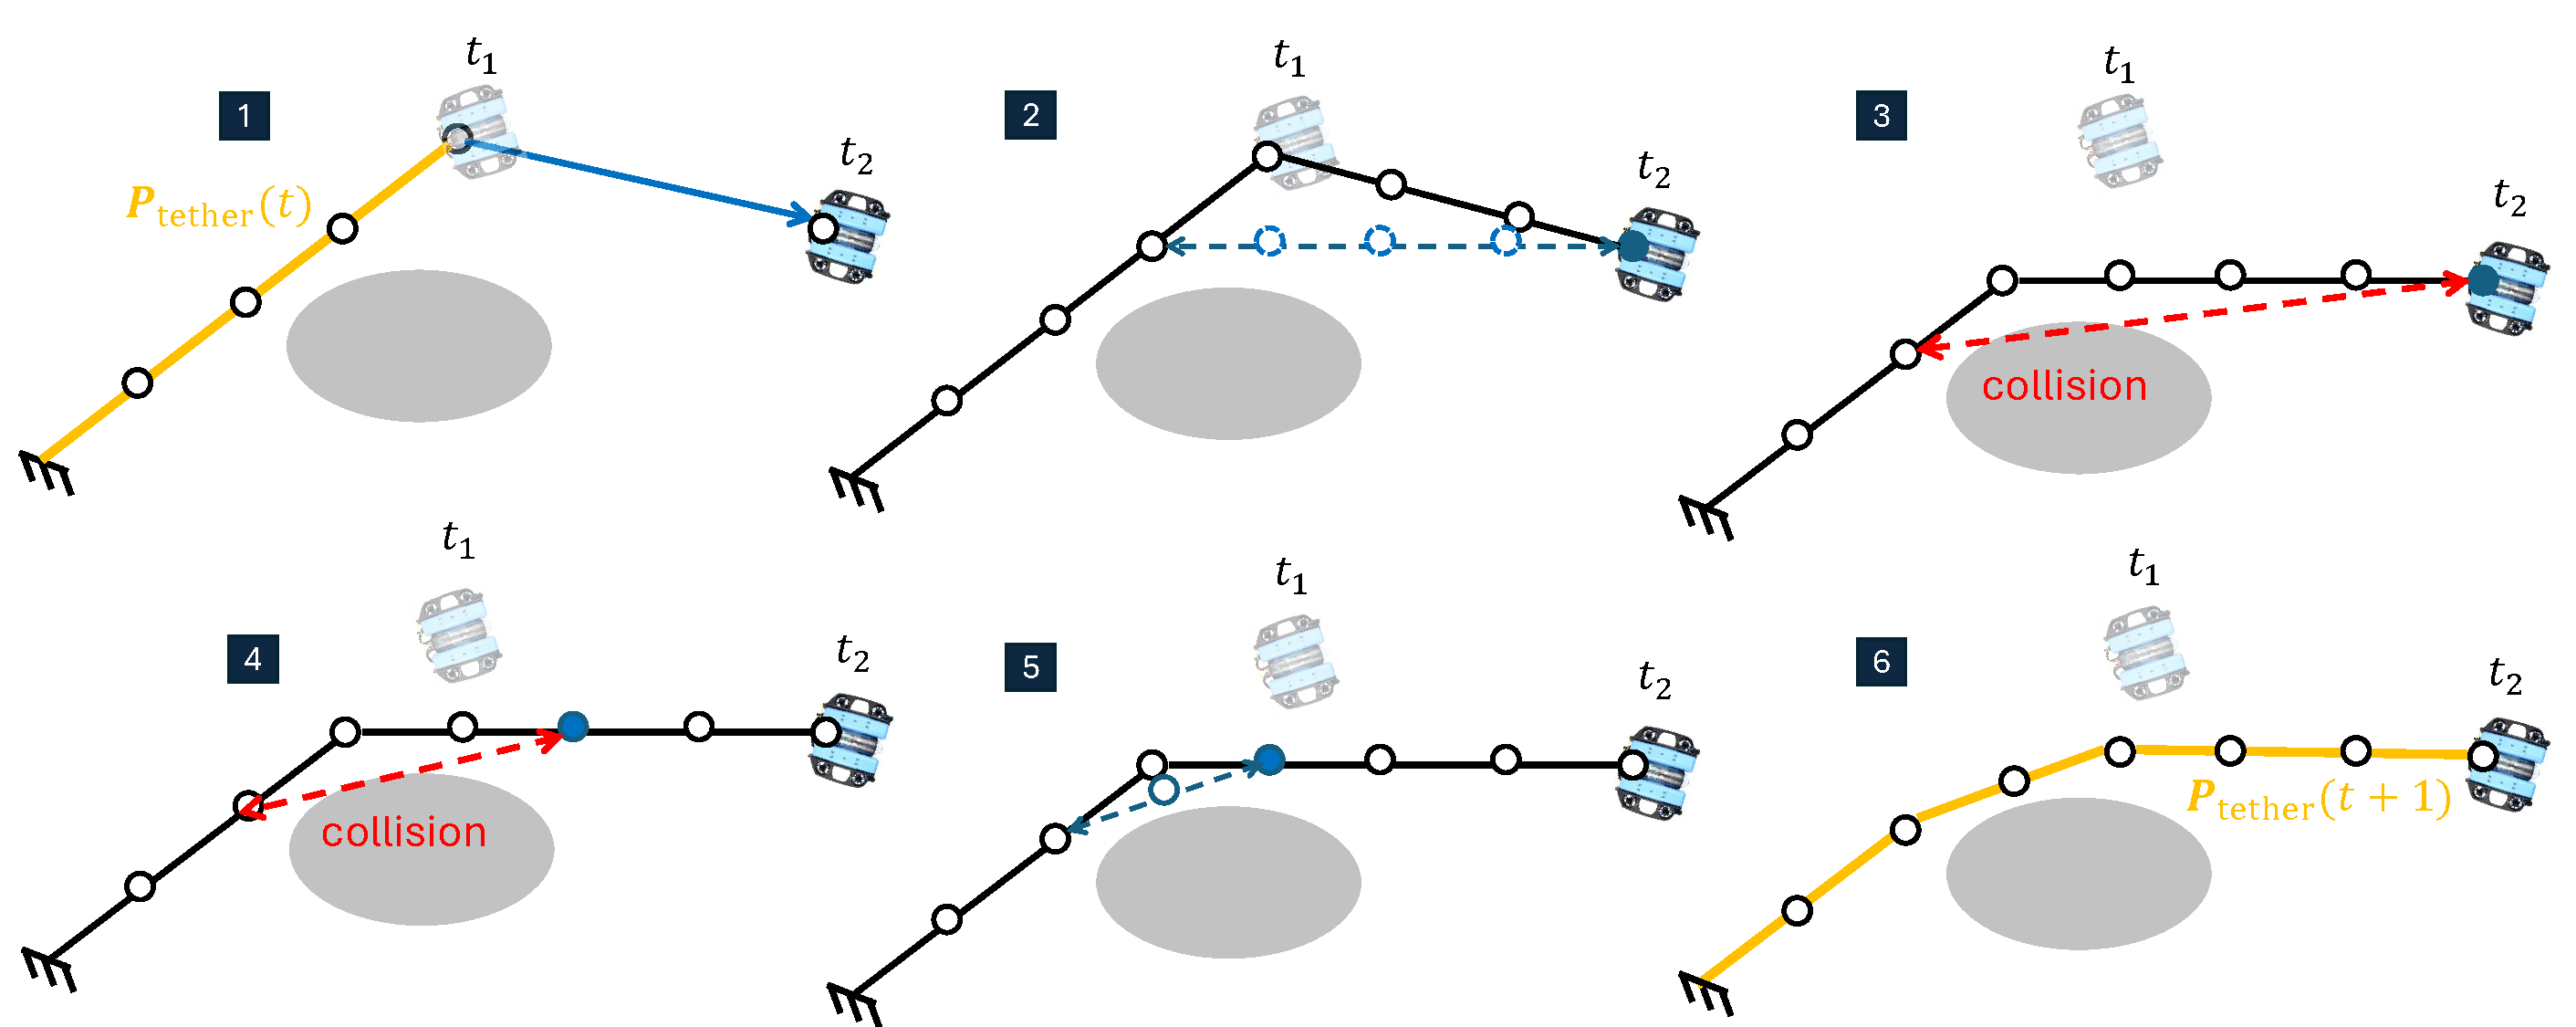
\includegraphics[width=1\linewidth]{EA-Planner/figures/tether_model.pdf}
    \caption{Tether shortcutting during \ac{ROV} motion from \( t_1 \) to \( t_2 \). (1) Initial tether with new \ac{ROV} position \( \mathbf{p}_{\text{rov}} \) appended; (2) Successful shortcut from the end node; (3) Collision encountered when attempting further shortcutting, prompting move to the next node; (4) Another collision detected from the new node; (5) Successful shortcut from a subsequent node; (6) Final tether configuration (yellow) after applying all feasible shortcuts.}
    \label{fig:tether}
\end{figure*}
%%%%%%%%%%%%%%%%%%%%%%%%



%%%%%%%%%%%%%%%%%%%%%%%%%%%
%%%%%%%%%%%%%%%%%%%%%%%%%%%
%%%%%% Tether Model Section
%%%%%%%%%%%%%%%%%%%%%%%%%%%
%%%%%%%%%%%%%%%%%%%%%%%%%%%
\section{Tether Modeling}
\label{sec:tether_model}
%Next, we introduce a computationally efficient kinematic \ac{ROV} tether model, inspired by the shortcutting algorithm used in the ropeRRT path planner \cite{roperrt}. In essence, the proposed model predicts the position of each node along the tether length based on \ac{ROV}'s relative pose to the base. 
%which simplifies sampled trajectories in a manner analogous to a rope tightening around an obstacle. The key assumption in the proposed model is that we assume a geometry-based constraint where the tether remains taut and fully stretched at all times.

 We introduce a computationally efficient kinematic tether model for tethered underwater vehicles. This model predicts the tether path, specifically the positions of each node along the tether's length, based on the \ac{ROV}'s relative pose to the base, and assumes a geometry-based constraint where the tether remains taut and fully stretched at all times. The main idea of the proposed tether model is inspired by the shortcutting algorithm of the ropeRRT path planner \cite{roperrt}, which simplifies sampled trajectories similar to a rope tightening around an obstacle. 


\subsection{Tether model description}
Let the tether path at time \( t \) be denoted by \( \mathbf{P}_{\mathrm{tether}}(t) = \{ \mathbf{p}_i(t) \}_{i=1}^{N} \), where each node \( \mathbf{p}_i(t) \in \mathbb{R}^3 \) represents the position of the \( i \)-th node in 3D space at time \( t \), and \( N \) is the total number of nodes in the tether path. The \ac{ROV} position at time \( t \), denoted by \( \mathbf{p}_{\mathrm{rov}}(t) \in \mathbb{R}^3 \), is appended at the end \( \mathbf{p}_{N+1}(t) \), ensuring that the \ac{ROV}'s position is included in the tether path. 

The proposed tether model iteratively optimizes the tether path via two primary mechanisms: shortcutting and pulling. %, as illustrated in Fig.~\ref{fig:tether}. 
%For each pair of nodes \( (\mathbf{p}_i(t), \mathbf{p}_j(t)) \) where \( i < j \), the algorithm attempts to shortcut the path segment between them.
Starting at the last node ($\mathbf{p}_j(t) = \mathbf{p}_{N}(t)$), the algorithm attempts to shortcut the path segment between each pair of nodes \( (\mathbf{p}_i(t), \mathbf{p}_j(t)) \) where \( i < j \).
If the line of sight between \( \mathbf{p}_i(t) \) and \( \mathbf{p}_j(t) \) is collision-free, as determined via an \ac{SDF} map (\( \mathcal{M}_{sdf} \)), the intermediate nodes are replaced with a straight segment sampled at known resolution \( \delta_n \). Conversely, if the line of sight encounters a collision, $j$ shifts to the preceding node, and the collision-free line of sight is rechecked. This process is repeated until a collision-free line of sight is found, and the intermediate nodes are then replaced. Fig.~\ref{fig:tether} illustrates an example of the shortcut operation. 

In the presence of non-convex obstacles, nodes might be positioned on or close to the obstacle following the shortcutting operation. Hence, if the shortcut is obstructed or the endpoint node \( \mathbf{p}_j(t) \) is in collision, the model applies a pulling operation. This operation essentially simulates disentanglement by moving \( \mathbf{p}_j(t) \) incrementally toward the tether endpoint \( \mathbf{p}_{N+1}(t) \), thus ensuring a collision-free updated path. This iterative process continues until no further shortcuts or pulling is feasible, resulting in an updated, taut, and obstacle-free tether path \( \mathbf{P}_{\mathrm{tether}}(t+1) \). Both the shortcutting and pulling operations are described in algorithm~\ref{alg:tether_optimization}.



%%%%%%%%%%%%%%%%%%%%%%%%%%%%%%%%%%%%%%%%%%
%%%%%%  Tether Model Algorithm  %%%%%%%%%
%%%%%%%%%%%%%%%%%%%%%%%%%%%%%%%%%%%%%%%%%%


\begin{algorithm}[t]
%\SetAlgoLined
\LinesNotNumbered  % Disable line numbers

\SetKwInOut{Input}{Require}
\SetKwInOut{Output}{Return}
\Input{
ROV position $\mathbf{p}_{\mathrm{rov}}(t)$, 
Tether path $\mathbf{P}_{\mathrm{tether}}(t)$, 
SDF map $\mathcal{M}_{sdf}$, 
parameters: $\delta_{n}$
}
\Output{Taut-tether at $t+1$ : $\mathbf{P}_{\mathrm{tether}}(t+1)$}
\BlankLine

\tcp{Extend tether path to include the current ROV position as the endpoint}
Append $\mathbf{p}_{\mathrm{rov}}(t)$ to $\mathbf{P}_{\mathrm{tether}}(t).end()$\;

%\tcp{Iterative shortcutting path segments by skipping intermediate nodes}
\tcp{Iterative shortcutting}
\For{$i \gets \mathrm{len}(\mathbf{P}_{\mathrm{tether}}(t)) - 1$ \textbf{to} $0$}{
    \For{$j \gets i - 1$ \textbf{to} $0$}{
        \tcp{Check if shortcutting the path is valid between nodes $i$ and $j$}
        \If{$\mathrm{checkShortcut}$($\mathbf{P}_{\mathrm{tether}}(t), i, j$)}{
            \tcp{Replace intermediate nodes $i-j$ }
            replaceNodes($\mathbf{P}_{\mathrm{tether}}(t)$, $i$, $j$, $\delta_{n}$)\;
        }
        \Else{
            \If{not $\mathrm{checkLineOfSight}$
            ($\mathcal{M}_{sdf}$, $\mathbf{P}_{\mathrm{tether}}(t)$)}{
                \tcp{Line of sight is blocked by obstacle, stop shortcutting}
                \textbf{break}\;
            }
            \If{$\mathrm{isInCollision}$($\mathcal{M}_{sdf}$, $\mathbf{P}_{\mathrm{tether}}(t)[j]$)}{
                \tcp{Pull node towards tether end}
                pullNode($\mathbf{P}_{\mathrm{tether}}(t)[j]$, $\mathbf{P}_{\mathrm{tether}}(t).end()$, $\delta_{n}$)\;
            }
        }
    }
}
\Return{$\mathbf{P}_{\mathrm{tether}}(t+1)$}\;
\caption{Taut-Tether Model}
\label{alg:tether_optimization}
\end{algorithm}




%%%%%%%%%%%%%%%%%%%%%%%%%%%
%%%%%%%%%%%%%%%%%%%%%%%%%%%
% Homotopy equivelance proof
%%%%%%%%%%%%%%%%%%%%%%%%%%%
%%%%%%%%%%%%%%%%%%%%%%%%%%%


% \subsection{Homotopic Equivalence of the Shortcutting-Based Tether Path}
% \label{sec:homotopy_proof}

% In this subsection, we demonstrate that the taut-tether path generated primarily through the shortcutting mechanism is homotopically equivalent to the Remotely Operated Vehicle's (ROV) actual trajectory. This argument focuses on the geometric simplification provided by shortcutting, assuming the tether behaves like a rope tightening around obstacles.

% \subsubsection{Preliminaries and Definitions}
% Let the ambient Euclidean space be $X = \mathbb{R}^3$. The static obstacle region, $O \subset X$, is a closed set. The \textbf{free configuration space} is defined as $C_{free} = X \setminus O$. A \textbf{path} in $C_{free}$ is a continuous function $\gamma: [0,1] \to C_{free}$.

% Two paths $\gamma_0, \gamma_1: [0,1] \to C_{free}$ sharing the same endpoints (i.e., $\gamma_0(0)=\gamma_1(0)$ and $\gamma_0(1)=\gamma_1(1)$) are said to be \textbf{homotopic in $C_{free}$} (denoted $\gamma_0 \sim \gamma_1$) if there exists a continuous function $H: [0,1] \times [0,1] \to C_{free}$, called a \textbf{homotopy}, such that:
% \begin{itemize}
%     \item $H(s,0) = \gamma_0(s)$ for all $s \in [0,1]$,
%     \item $H(s,1) = \gamma_1(s)$ for all $s \in [0,1]$,
%     \item $H(0,\tau) = \gamma_0(0)$ for all $\tau \in [0,1]$ (startpoints fixed),
%     \item $H(1,\tau) = \gamma_0(1)$ for all $\tau \in [0,1]$ (endpoints fixed).
% \end{itemize}
% Let $p_A \in C_{free}$ denote the fixed anchor point of the tether and $p_R(t) \in C_{free}$ be the ROV's position at time $t$. The actual continuous trajectory of the ROV up to time $t$ is a path $\Gamma_{\mathrm{rov}}: [0,1] \to C_{free}$, with $\Gamma_{\mathrm{rov}}(0) = p_A$ (assuming the path starts at the anchor for simplicity) and $\Gamma_{\mathrm{rov}}(1) = p_R(t)$.

% A \textbf{piecewise linear (PL) path}, $\mathbf{P}$, connecting $p_A$ to $p_R(t)$ is defined by an ordered sequence of $N+1$ vertices $(v_0, v_1, \ldots, v_N)$ where $v_0=p_A$, $v_N=p_R(t)$, and each $v_k \in C_{free}$. The path consists of line segments $L(v_k, v_{k+1}) = \{ (1-s)v_k + s v_{k+1} \mid s \in [0,1] \}$. For $\mathbf{P}$ to be a path in $C_{free}$, each segment $L(v_k, v_{k+1})$ must be entirely contained in $C_{free}$.

% \subsubsection{Initial Tether Path and Shortcutting as a Homotopy}
% Let $\mathbf{P}_{init}(t)$ be an initial PL path representing the tether before shortcutting optimization at time $t$. This path connects $p_A$ to $p_R(t)$ and is assumed to be a PL approximation of $\Gamma_{\mathrm{rov}}$ lying in $C_{free}$. It is a standard result in algebraic topology that $\Gamma_{\mathrm{rov}} \sim \mathbf{P}_{init}(t)$ if $\mathbf{P}_{init}(t)$ is a sufficiently fine approximation.

% The shortcutting mechanism iteratively refines a PL path. Let $\mathbf{P}_{k} = (v_0, \ldots, v_M)$ be the PL tether path at iteration $k$. A shortcutting step selects two non-consecutive vertices $v_i, v_j \in \mathbf{P}_{k}$ (where $i < j-1$). Let $\sigma_{old}$ be the subpath of $\mathbf{P}_{k}$ from $v_i$ to $v_j$, and let $\sigma_{new}$ be the straight-line segment $L(v_i, v_j)$. If $\sigma_{new} \subset C_{free}$ (i.e., the line of sight is collision-free), the path $\mathbf{P}_{k+1}$ is formed by replacing $\sigma_{old}$ with $\sigma_{new}$.

% \textbf{Claim:} If $\sigma_{new} \subset C_{free}$, then $\sigma_{old} \sim \sigma_{new}$ in $C_{free}$ relative to their common endpoints $v_i$ and $v_j$.

% \textit{Proof of Claim:}
% The tether model is "analogous to a rope tightening around an obstacle." When a flexible rope segment, initially following $\sigma_{old} \subset C_{free}$, is pulled taut between $v_i$ and $v_j$, and the direct path $\sigma_{new}$ is also in $C_{free}$, the rope physically deforms into $\sigma_{new}$ by moving exclusively through $C_{free}$.
% This continuous deformation can be represented by a homotopy. Let $\sigma_{old}(s)$ parameterize the PL path $\sigma_{old}$ for $s \in [0,1]$, and $\sigma_{new}(s) = (1-s)v_i + s v_j$ parameterize the segment $\sigma_{new}$. A straight-line homotopy is $H(s, \tau) = (1-\tau)\sigma_{old}(s) + \tau\sigma_{new}(s)$ for $s, \tau \in [0,1]$.
% The "rope tightening" analogy implies that if $\sigma_{new} \subset C_{free}$, then the entire region swept by the deformation from $\sigma_{old}$ to $\sigma_{new}$ is also contained in $C_{free}$. Thus, $H(s, \tau) \in C_{free}$ for all $s, \tau$. This ensures that $\sigma_{old} \sim \sigma_{new}$ in $C_{free}$.
% Since $\mathbf{P}_{k+1}$ is obtained from $\mathbf{P}_{k}$ by substituting $\sigma_{old}$ with a homotopic segment $\sigma_{new}$, it follows that $\mathbf{P}_{k} \sim \mathbf{P}_{k+1}$.
% \hfill $\qed$

% \subsubsection{Iterative Application and Final Equivalence}
% The shortcutting algorithm generates a sequence of PL paths $\mathbf{P}_{init}(t) = \mathbf{P}_0, \mathbf{P}_1, \ldots, \mathbf{P}_{final}$, where $\mathbf{P}_{final}$ is the resulting taut-tether path, denoted $\mathbf{P}^{tether}(t)$. Since each step is a homotopy, $\mathbf{P}_0 \sim \mathbf{P}_1 \sim \ldots \sim \mathbf{P}_{final}$. By the transitivity of the homotopy relation, $\mathbf{P}_{init}(t) \sim \mathbf{P}^{tether}(t)$.

% Given that $\Gamma_{\mathrm{rov}} \sim \mathbf{P}_{init}(t)$, and $\mathbf{P}_{init}(t) \sim \mathbf{P}^{tether}(t)$, we conclude by transitivity that:
% $$ \Gamma_{\mathrm{rov}} \sim \mathbf{P}^{tether}(t) $$
% Thus, the taut-tether path $\mathbf{P}^{tether}(t)$, resulting from the shortcutting operations, is homotopically equivalent to the ROV's actual trajectory $\Gamma_{\mathrm{rov}}$ within the free configuration space $C_{free}$. The shortcutting process simplifies the path to a tighter representative within its original homotopy class with respect to the obstacles.



%%%%%%%%%%%%%%%%%%%%%%%%%%%%%%%%%%%%%%%%%%
%%%%%%%%%%%%%%%%%%%%%%%%%%%%%%%%%%%%%%%%%%
%%%%%%%%%%%%%%%%%%%%%%%%%%%%%%%%%%%%%%%%%%



%%%%%%%%%%%%%%%%%%%%%%%%%%%
%%%%% REACT Planner %%%%%%
%%%%%%%%%%%%%%%%%%%%%%%%%%%
% \begin{algorithm}[t]
% \LinesNotNumbered  % Disable line numbers

% \SetKwInOut{Input}{Input}
% \SetKwInOut{Output}{Return}
% \Input{
% Waypoints $\mathbf{W}$, 
% Maximum tether length $L_{\max}$, 
% Current tether path $\mathbf{P}_{\mathrm{tether}}(t)$, 
% Current ROV position $\mathbf{p}_{\text{rov}}(t)$, 
% Current waypoint index $k$, $d_{\mathrm{thresh}}$}

% \Output{Target waypoint for the controller $\mathbf{p}_{\text{target}}$}
% \BlankLine

% Compute $L_{\text{tether}}(t)$ 

% \If{$L_{\mathrm{tether}}(t) > L_{\max}$ \textbf{and not} $search\_safe\_path$}{
%     $search\_safe\_path \gets$ True\; \tcp{Activate recovery mode}
%     $\mathbf{P}_{\text{recovery}} \gets \text{searchAlternativePath}(\mathbf{P}_{\mathrm{tether}}(t), \mathbf{W}[k], L_{\max})$\; \tcp{Find path within tether limits}
%     $\mathbf{P}_{\text{safe}} \gets \text{refineRecoveryPath}(\mathbf{P}_{\text{recovery}})$\; \tcp{Optimize the recovery path}
%     $is\_path\_safe$ $\gets \text{checkPathValidity}(\mathbf{P}_{\text{safe}})$\; \tcp{Check if recovery path is valid}
%     $safe\_path\_index$ $\gets 0$\; \tcp{Start from the beginning of the recovery path}
% }

% \If{$search\_safe\_path$ \textbf{and} $is\_path\_safe$}{
%     $\mathbf{p}_{\text{target}} \gets \text{getPointAlongPath}(\mathbf{P}_{\text{safe}}, \; safe\_path\_index)$\; \tcp{Get target from recovery path}
%     \If{$\|\mathbf{p}_{\mathrm{rov}}(t) - \mathbf{p}_{\mathrm{target}}\| < d_{\mathrm{thresh}}$}{
%         $safe\_path\_index \gets safe\_path\_index + 1$\; \tcp{Advance to next point}
%     }
%     \If{$safe\_path\_index \ge |\mathbf{P}_{\text{safe}}|$}{
%         $search\_safe\_path \gets$ False\; \tcp{Recovery complete}
%         $\mathbf{p}_{\text{target}} \gets \mathbf{W}[k]$\; \tcp{Resume wp tracking}
%     }
% }
% % hey sorry mohit, i didnt realize you were editing this
% \Else{
%     $search\_safe\_path \gets$ False\; \tcp{Reset recovery}
%     $\mathbf{p}_{\mathrm{target}} \gets \mathbf{W}[k]$\; \tcp{Default to current wp}

%     \If{$\|\mathbf{p}_{\mathrm{rov}}(t) - \mathbf{p}_{\mathrm{target}}\| < d_{\mathrm{thresh}}$}{
%          $k \gets k + 1$\; \tcp{Advance to next wp}
%     }
% }
% \Return{$\mathbf{p}_{\mathrm{target}}$}\;
% \caption{Real-time Entanglement-Aware Path Planning}
% \label{alg:main_loop}
% \end{algorithm}










%%%%%%%%%%%%%%%%%%%%%%%%%%%%%%%%%
%% Alg. 3 Recovery Path  Algorithm %%%
%%%%%%%%%%%%%%%%%%%%%%%%%%%%%%%%%

% \begin{algorithm}[b]
% \LinesNotNumbered  % Disable line numbers
% \SetKwInOut{Input}{Input}
% \SetKwInOut{Output}{Return}
% \Input{
% Current tether $\mathbf{P}(t)$,
% Goal waypoint $\mathbf{p}_{\text{goal}}$,
% Maximum length $L_{\max}$
% }
% \Output{Recovery path segment $\mathbf{P}_{\text{recovery}}$}
% \BlankLine
%  $best\_path$ $\gets$ None\; \\
%  $prev\_len$ $\gets \infty$\; \\
%  $found\_suitable$ $\gets$ False\; \\
% \For{$i \gets |\mathbf{P}(t)| - 3$ \textbf{downto} 3}{
%     $\mathbf{P}_{\text{candidate}} \gets \text{generatePath}(i, \mathbf{P}(t), \mathbf{p}_{\text{goal}})$\; \\
%     $L_{\text{candidate}} \gets \text{computeLength}(i, \mathbf{P}(t), \mathbf{P}_{\text{candidate}})$\;\\
%     \If{$L_{\text{candidate}} < 0.7L_{\max}$} %\textbf{and} $L_{\text{candidate}} < 0.65 \cdot \text{prev\_len}$}
%     {
%           $best\_path$ $\gets \text{ExtractSegment}(i+2, \mathbf{P}(t))$\;
%          found\_suitable $\gets$ True\;
%          \textbf{break}\;
%     }
%      $prev\_len$ $\gets \text{computeLength}(i-3, \mathbf{P}(t), \text{generatePath}(i-3, \mathbf{P}(t), \mathbf{p}_{\text{goal}}))$\;
% }
% \If{\textbf{not} found\_suitable}{
%     $\mathbf{p}_{\text{rov}} \gets \mathbf{P}(t)[|\mathbf{P}(t)|-1]$\; \tcp{Fallback}
%     $\mathbf{P}_{\text{recovery}}$ $\gets \text{planShortestPath}(\mathbf{p}_{\text{rov}}, \mathbf{p}_{\text{goal}})$\;
% }
% \Return{$\mathbf{P}_{\text{recovery}}$}\;
% \caption{Search Alternative Recovery Path}
% \label{alg:search_alternative}
% \end{algorithm}

%%%%%%%%%%%%%%%%%%%%%%%%%%%%%%%%%%%%%%%%%%
%%%%%%%%%%%%%%%%%%%%%%%%%%%%%%%%%%%%%%%%%%
%%%%%%%%%%%%%%%%%%%%%%%%%%%%%%%%%%%%%%%%%%

%%%%%%%%%%%%%%%%%%%%%%%%%%%
%%%%% REACT Planner %%%%%%
%%%%%%%%%%%%%%%%%%%%%%%%%%%
%%%%%%%%%%%%%%%%%%%%%%%%%%%
%%%%% REACT Planner %%%%%%
%%%%%%%%%%%%%%%%%%%%%%%%%%%
\begin{algorithm}[t]
\LinesNotNumbered  % Disable line numbers
\SetKwInOut{Input}{Input}
\SetKwInOut{Output}{Output}
\Input{
Waypoints $\mathbf{W}$, 
Maximum tether length $L_{\max}$, 
Current tether path $\mathbf{P}_{\mathrm{tether}}(t)$, 
Current ROV position $\mathbf{p}_{\text{rov}}(t)$, 
Current waypoint index $k$
}
\Output{Target position $\mathbf{p}_{\text{target}}$ for ROV controller}
\BlankLine
\tcp{Entanglement Detection}
$L_{\text{tether}}(t) \gets \text{computeLength}(\mathbf{P}_{\mathrm{tether}}(t))$\;
\BlankLine
\If{$L_{\mathrm{tether}}(t) > L_{\max}$}{
    \tcp{De-entanglement Mode: Search for recovery path}
    $\mathbf{P}_{\text{safe}} \gets \text{deEntanglementPathSearch}(\mathbf{P}_{\mathrm{tether}}(t), \mathbf{W}[k], L_{\max})$\;
    \BlankLine
    % \If{$\mathbf{P}_{\text{safe}}$ is valid}{
    %     $\mathbf{p}_{\text{target}} \gets \text{followRecoveryPath}(\mathbf{P}_{\text{safe}}, \mathbf{p}_{\text{rov}}(t))$\;
    % }
    % \Else{
    %     $\mathbf{p}_{\text{target}} \gets \text{emergencyFallback}(\mathbf{p}_{\text{rov}}(t))$\; \tcp{wait}
    % }
}
\Else{
    \tcp{Normal Waypoint Following Mode}
    $\mathbf{p}_{\text{target}} \gets \mathbf{W}[k]$\;
    \BlankLine
    \If{ROV reached current waypoint}{
        $k \gets k + 1$\; \tcp{Advance to next waypoint}
    }
}
\BlankLine
\Return{$\mathbf{p}_{\text{target}}$}\;
\caption{Real-time Entanglement-Aware Path Planning}
\label{alg:main_loop}
\end{algorithm}





%%%%%%%%%%%%%%%%%%%%%%%%%%%%%%%%%
%% Alg. 3 Recovery Path Algorithm %%%
%%%%%%%%%%%%%%%%%%%%%%%%%%%%%%%%%
\begin{algorithm}[t]
\LinesNotNumbered  % Disable line numbers
\SetKwInOut{Input}{Input}
\SetKwInOut{Output}{Output}
\Input{
Current tether $\mathbf{P}_{\text{tether}}(t)$,
Target waypoint $\mathbf{W}[k]$,
Maximum length $L_{\max}$
}
\Output{Recovery path $\mathbf{P}_{\text{recovery}}$ with segments $\mathbf{P}_{\text{r}1}$ and $\mathbf{P}_{\text{r}2}$}
\BlankLine
 $\mathbf{p}_{\text{pivot}} \gets$ None\; \\
 $found\_feasible$ $\gets$ False\; \\
 \BlankLine
 \tcp{Backward recovery search along tether trajectory}
\For{$i \gets |\mathbf{P}_{\text{tether}}(t)| - 2$ \textbf{downto} 1}{
    $\mathbf{p}_{\text{candidate}} \gets \mathbf{P}_{\text{tether}}(t)[i]$\; \\
    $\mathbf{P}_{\text{c}} \gets \text{planShortestPath}(\mathbf{p}_{\text{candidate}}, \mathbf{W}[k])$\; \\
    \BlankLine
    \tcp{Create candidate path and simulate tether using tether model}
    $\mathbf{P}_{\text{candidate\_path}} \gets \text{extractSegment}(0, i, \mathbf{P}_{\text{tether}}(t)) \cup \mathbf{P}_{\text{c}}$\; \\
    $\mathbf{P}_{\text{tether}}(t+1) \gets \text{tetherModel}(\mathbf{P}_{\text{candidate\_path}})$\; \\
    $L_{\text{new}} \gets \text{computeLength}(\mathbf{P}_{\text{tether}}(t+1))$\; \\
    \BlankLine
    \If{$L_{\text{new}} \leq L_{\max}$}{
        $\mathbf{p}_{\text{pivot}} \gets \mathbf{p}_{\text{candidate}}$\; \\
        $\mathbf{P}_{\text{r}1} \gets \text{extractSegment}(0, i, \mathbf{P}_{\text{tether}}(t))$\; \\
        $\mathbf{P}_{\text{r}2} \gets \mathbf{P}_{\text{c}}$\; \\
        $found\_feasible \gets$ True\;
        \textbf{break}\;
    }
}
\BlankLine
\If{\textbf{not} found\_feasible}{
    \tcp{Fallback: treat tether constraint as soft constraint}
    $\mathbf{p}_{\text{pivot}} \gets \mathbf{p}_{\text{rov}}(t)$\; \tcp{Current ROV position}
    $\mathbf{P}_{\text{r}1} \gets \emptyset$\; \\
    $\mathbf{P}_{\text{r}2} \gets \text{planShortestPath}(\mathbf{p}_{\text{pivot}}, \mathbf{W}[k])$\;
}
\BlankLine
$\mathbf{P}_{\text{recovery}} \gets \mathbf{P}_{\text{r}1} \cup \mathbf{P}_{\text{r}2}$\;
\Return{$\mathbf{P}_{\text{recovery}}$}\;
\caption{De-entanglement Path Search}
\label{alg:search_alternative}
\end{algorithm}





%%%%%%%%%%%%%%%%%%%%%%%%%%%
%% Refine Path  Algorithm
%%%%%%%%%%%%%%%%%%%%%%%%%%%
% \begin{algorithm}[t]
% \LinesNotNumbered  % Disable line numbers
% \SetKwInOut{Input}{Input}
% \SetKwInOut{Output}{Return}
% \Input{
%     Recovery path $\mathbf{P}_{\text{recovery}}$;\\
%     Offset distance $\delta_{\text{offset}}$;\\
%     Sampling distance $\delta_{\text{sample}}$
% }
% \Output{Refined safe path $\mathbf{P}_{\text{safe}}$}
% \BlankLine
% $\mathbf{P}_{\text{offset}} \gets \text{tetherPathOffset}(\mathbf{P}_{\text{recovery}}, \delta_{\text{offset}})$\;
% \\
% $\mathbf{P}_{\text{sampled}} \gets \text{perturbTetherPath}(\mathbf{P}_{\text{offset}}, \delta_{\text{sample}})$\;
% \\
% $\mathbf{P}_{\text{safe}} \gets \text{smoothTetherPath}(\mathbf{P}_{\text{sampled}})$\;
% \\
% \Return{$\mathbf{P}_{\text{safe}}$}\;
% \caption{Refine Recovery Path}
% \label{alg:refine_path}
% \end{algorithm}


%%%%%%%%%%%%%%
%%%%%%%%%%%%%%
%%%%%%%%%%%%%%

%%%%%%%%%%%%%%%%%%%%%%%%%%%
%%%%%%%%%%%%%%%%%%%%%%%%%%%
%%%%%%% PLANNER %%%%%%%%%
%%%%%%%%%%%%%%%%%%%%%%%%%%
%%%%%%%%%%%%%%%%%%%%%%%%%%





\section{Entanglement-Aware Path Planner}
\label{sec:planner}

Next, we present the entanglement-aware path planner. In essence, it is a local planner designed to address the real-time entanglement free path-finding problem for autonomous systems operating with a tether. 
The planner runs in an online manner, continuously monitoring the tether configuration and adapting the \ac{ROV}'s path to avoid exceeding the maximum allowable tether length, \( L_{\mathrm{max}} \), while ensuring safe, collision-free motion towards a sequence of reference waypoints.

At each time step \( t \), the planner obtains the estimated tether path  $\mathbf{P}_{\mathrm{tether}}(t)$ from the tether model. The planner also maintains a list of reference waypoints \( \mathbf{W} = \{\mathbf{p}_{\text{waypoint}}(k)\}_{k=1}^{M} \), where \( \mathbf{p}_{\text{waypoint}}(k) \in \mathbb{R}^3 \) denotes the \( k \)-th target waypoint. The current tether length \( L_{\text{tether}}(t) \) is computed by summing the Euclidean distances between consecutive tether points, i.e., \( L_{\text{tether}}(t) = \sum_{i=1}^{N-1} \| \mathbf{p}_i(t) - \mathbf{p}_{i+1}(t) \| \), and is subsequently compared to the predefined maximum allowable length \( L_{\text{max}} \), to activate the re-planner.

\subsection{Nominal Operation}
If the tether length constraint is satisfied, i.e., \( L_{\text{tether}}(t) \leq L_{\text{max}} \), the planner operates in its nominal mode. The planner identifies the next reference waypoint \( \mathbf{p}_{\text{waypoint}}(k) \) from the list \( \mathbf{W} \) (not yet reached) and directs the \ac{ROV} towards it. The system proceeds sequentially through the waypoints as long as the tether constraint remains satisfied.



\subsection{De-entaglement path search}

% If the tether length exceeds the maximum allowed limit \( L_{\text{tether}}(t) > L_{\text{max}} \), the entanglement avoidance strategy is activated. This strategy aims to guide the \ac{ROV} along a temporary recovery path for tether detangling before resuming navigation towards the original target waypoint.
% %
% The planner initiates this search for a suitable recovery path by iteratively evaluating potential detangle paths based on the current tether path \( \mathbf{P}_{\mathrm{tether}}(t) \). Starting from the second-last node (\( \mathbf{p}_{N-1}(t) \)) and moving back towards the anchor point \( \mathbf{p}_1(t) \), the planner considers each node \( \mathbf{p}_i(t) \) as a potential pivot point -- \ac{ROV}'s returning point --. For each \( i \), a candidate alternative trajectory is implicitly generated, consisting of the segment from the \ac{ROV} back to \( \mathbf{p}_i(t) \) followed by a newly planned path segment from \( \mathbf{p}_i(t) \) to the current target waypoint \( \mathbf{p}_{\text{waypoint}}(k) \). The planner also computes the estimated length of this candidate alternative tether configuration.

% A recovery path is selected based on a length criteria: the planner seeks a pivot point \( \mathbf{p}_i(t) \) such that the corresponding alternative path length is significantly shorter than \( L_{\text{max}} \) (e.g., \( < 0.7 L_{\text{max}} \)) and offers substantial improvement compared to alternatives generated using nearby pivot points (e.g., \( \mathbf{p}_{i-3}(t) \)). Once such an index \( i \) is found, the recovery path segment \( \mathbf{P}_{\text{recovery}} \) is defined as the portion of the current tether from the \ac{ROV} back to a point slightly further back along the tether, specifically \( \mathbf{p}_{i+2}(t) \). This segment represents the initial trajectory the \ac{ROV} must follow to begin resolving the entanglement. If no suitable recovery path is found during the backward search, a direct path from the \ac{ROV}'s current position to the goal waypoint is generated as a fallback. This recovery path search process is illustrated in Fig. \ref{fig:planner_search}.  
If the tether length exceeds the maximum allowed limit $L_{\text{tether}}(t) > L_{\text{max}}$, the entanglement avoidance strategy is activated. This strategy aims to guide the ROV along a temporary recovery path for tether detangling before resuming navigation towards the original target waypoint.

The planner initiates a backward recovery search along the tether trajectory $\mathbf{P}_{\mathrm{tether}}(t)$ by iteratively evaluating potential pivot points. Starting from the second-last node of the current tether path and moving backwards towards the anchor point, the planner considers each node $\mathbf{p}_i(t)$ as a potential pivot point. For each candidate pivot point $\mathbf{p}_i(t)$, the planner constructs a candidate path $\mathbf{P}_c$ by combining the tether segment from the anchor up to the pivot point $\mathbf{p}_i(t)$ with the shortest path from the pivot point to the current target waypoint $\mathbf{W}[k]$.

To accurately assess the feasibility of this candidate configuration, the planner employs the tether model \ref{alg:tether_optimization} that simulates the physical behavior of the taut tether. The candidate path is fed into the tether model function, which computes the equivalent taut tether path at time $t+1$ $\mathbf{P}_{\mathrm{tether}}(t+1)$. The total length $L_{\text{new}}$ is then computed from this simulated tether path.

The first pivot point that yields a feasible solution—where the simulated tether length satisfies $L_{\text{new}} \leq L_{\text{max}}$—is selected as the recovery strategy. The resulting recovery path $\mathbf{P}_{\text{recovery}}$ is then constructed with two segments: $\mathbf{P}_{\text{r}1}$, consisting of the tether segment from the anchor up to the selected pivot point, and $\mathbf{P}_{\text{r}2}$, representing the shortest path from the pivot point to the target waypoint. This approach prioritizes finding the most recent (furthest along the tether) feasible pivot point, minimizing the distance the \ac{ROV} needs to backtrack while ensuring realistic tether constraint satisfaction through physics-based simulation.

If no suitable pivot point is found during the backward search, the planner falls back to treating the tether constraint as a soft constraint and proceeds directly towards the target waypoint, accepting that the tether length may temporarily exceed $L_{\text{max}}$. This recovery path search process is illustrated in Fig. \ref{fig:planner_search}.







%%%%%%%%%%%%%%%%%%%%%%%%%
%%%% Figure : Planner search 
%%%%%%%%%%%%%%%%%%%%%%%%
%%%%%%%%%%%%%%%%%%%%%%%%
% \begin{figure*}[h]
%     \centering
%     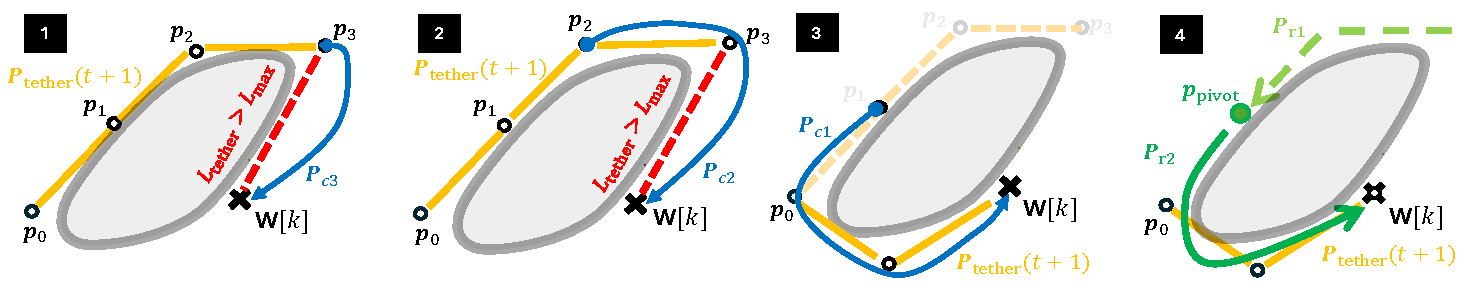
\includegraphics[width=\textwidth]{EA-Planner/figures/planner_newest.pdf}
%     \caption{De-entanglement path search process. 
%     (1) Entanglement detection: following the path from node \( \mathbf{p}_3 \), denoted as \( \mathbf{P}_{c_3} \), causes the tether length \( L_{\text{tether}} \) to exceed the maximum allowed length \( L_{\text{max}} \); 
%     (2) a backward recovery search is initiated from node \( \mathbf{p}_2 \) along the tether trajectory \( \mathbf{P}_{\mathrm{tether}}(t) \), but the resulting path yields no improvement in tether length; 
%     (3) continuing the search further back to node \( \mathbf{p}_1 \) leads to a feasible path and an updated, valid tether configuration; 
%     (4) the final planned safe path \( \mathbf{P}_{\text{safe}} \) (green), which satisfies the tether constraint (\( L_{\text{tether}} \leq L_{\text{max}} \)), consists of two segments: \( \mathbf{P}_{\text{safe},1} \), the part of the tether path up to node \( \mathbf{p}_1 \) (also \( \mathbf{p}_{\text{pivot}} \)), and \( \mathbf{P}_{\text{safe},2} \), the shortest path from \( \mathbf{p}_2 \) towards the target waypoint \( \mathbf{W}[k] \), ensuring an entanglement-free tether path $\mathbf{P}_{\mathrm{tether}}(t+1)$.}
%     \label{fig:planner_search}
% \end{figure*}
%%%%%%%%%%%%%%%%
%%%%%%%%%%%%%%%%
\begin{figure*}[h]
    \centering
    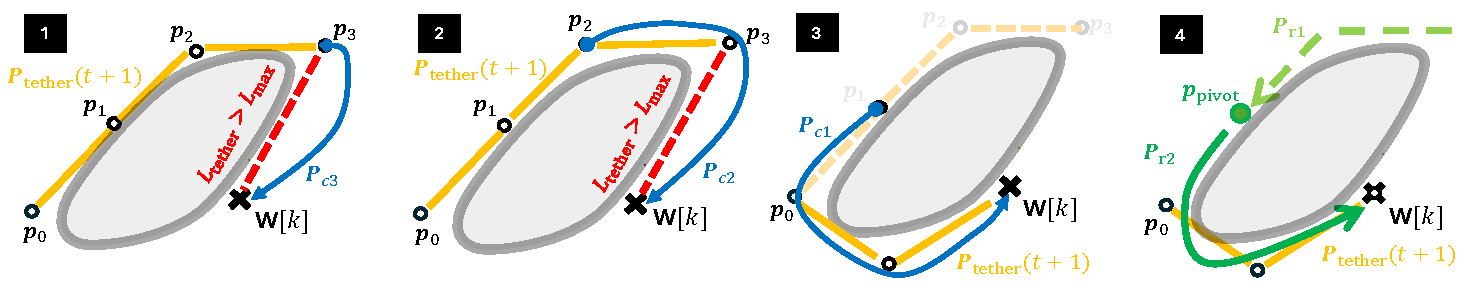
\includegraphics[width=\textwidth]{EA-Planner/figures/planner_newest.pdf}
    \caption{De-entanglement path search process. 
    (1) Entanglement detection: following the path from node \( \mathbf{p}_3 \), denoted as \( \mathbf{P}_{c_3} \), causes the tether length \( L_{\text{tether}} \) to exceed the maximum allowed length \( L_{\text{max}} \); 
    (2) a backward recovery search is initiated from node \( \mathbf{p}_2 \) along the tether trajectory \( \mathbf{P}_{\mathrm{tether}}(t) \). The candidate path \( \mathbf{P}_{c_2} \) (tether segment to \( \mathbf{p}_2 \) plus shortest path to waypoint) is evaluated using the tether model, but the resulting simulated tether length yields no feasible solution; 
    (3) continuing the search further back to node \( \mathbf{p}_1 \) leads to a feasible path. The candidate path \( \mathbf{P}_{c_1} \) produces a simulated tether configuration that satisfies the length constraint; 
    (4) the final planned recovery path \( \mathbf{P}_{\text{recovery}} \) (green), which satisfies the tether constraint (\( L_{\text{tether}} \leq L_{\text{max}} \)), consists of two segments: \( \mathbf{P}_{\text{r}1} \), the part of the tether path up to node \( \mathbf{p}_1 \) (also \( \mathbf{p}_{\text{pivot}} \)), and \( \mathbf{P}_{\text{r}2} \), the shortest path from \( \mathbf{p}_1 \) towards the target waypoint \( \mathbf{W}[k] \), ensuring an entanglement-free tether path $\mathbf{P}_{\mathrm{tether}}(t+1)$.}
    \label{fig:planner_search}
\end{figure*}



\subsection{Recovery Path Refinement and Execution}
The initially selected recovery path \( \mathbf{P}_{\text{recovery}} \) undergoes further refinement to enhance safety and smoothness before execution. This involves several steps:
\begin{enumerate}
    \item Centroid Offsetting: Points along \( \mathbf{P}_{\text{recovery}} \) are pushed slightly outwards, away from the path's geometric centroid, to increase clearance from potential obstacles near the path's center.
    \item Random Sampling Perturbation: Points are locally perturbed by sampling in random directions, seeking nearby collision-free states to potentially escape minor constraint violations or local minima.
    \item Polynomial Smoothing: A third order polynomial function is fitted to segments of the path to reduce sharp turns and generate a  smoother reference trajectory.
\end{enumerate}
The resulting refined path is denoted as \( \mathbf{P}_{\text{safe}} \). The planner then checks if \( \mathbf{P}_{\text{safe}} \) is collision-free. The core logic can be summarized in the following algorithms. Algorithm~\ref{alg:main_loop} outlines the main planning cycle, Algorithm~\ref{alg:search_alternative} details the search for the recovery path.














%%%%%%%%%%%%%%%%%%%%%%%%%%%%%%%%%%%%%%%%%%
%%%%%%%%%%%%%%%%%%%%%%%%%%%%%%%%%%%%%%%%%%
%%%%%%%%%%%%%%%%%%%%%%%%%%%%%%%%%%%%%%%%%%













 % 1.5 pages
\section{Simulations Experiments}
\label{sec:simulationexperiments}


This section presents the experimental results of the simulations of our proposed \ac{REACT} method. The entire framework is implemented in C++ to ensure computational efficiency and is integrated with ROS to facilitate modularity and deployment on real-world robots. Furthermore, the \ac{OMPL} library \cite{ompl} was utilized to compute the shortest paths using the RRT* algorithm.  


\subsection{Simulation experimental setup }
The path planner is implemented for a BlueROV2. A \ac{MPC} approach is used to account for model constraints and provide the optimal control input $\mathbf{u}^{ref} \in \mathbb{R}^4$, where $\mathbf{u}^{ref} = [F_x, F_y, F_z, M_z]^T$ represents the forces in the $X$, $Y$, and $Z$ directions, and the moment about the $Z$-axis. The goal is to follow the desired reference trajectory $\mathbf{x}^{ref} \in \mathbb{R}^6$, where $\mathbf{x}^{ref} = [x_{ref}, y_{ref}, z_{ref}, \psi_{ref}]^T$ contains the reference position ($x_{ref}$, $y_{ref}$, $z_{ref}$) and the reference yaw angle $\psi_{ref}$.

The entanglement-aware path planner provides $\mathbf{x}^{ref}$ in real time, ensuring the BlueROV2 avoids obstacles while following the desired trajectory. For further details about the controller and model, the reader is referred to \cite{amergp}.

%\subsection{Results}
We perform a comparative analysis of the proposed \ac{REACT} method and a baseline conventional \ac{CPP} (FC-Planner \cite{feng2024fc}), which does not contain explicit handling of entanglement. 

The simulation setup consists of a pipe structure represented by an underwater pipe model from \cite{feng2024fc}. The simulated onboard camera featured a field of view of 70 degrees. The tether constraint was defined by a maximum allowed tether length of $L_{max}$ = 10.0 meters.

Environmental coverage was evaluated geometrically similar to \cite{amer2023visual}. At each subsampled time step, the position and orientation of the camera were used to determine which triangles in the environment mesh were visible. A triangle was marked as visible if its centroid was within the inspection range, its surface normal faced the camera, and its projection lay within the camera's field of view. Over time, the set of all uniquely observed triangles was accumulated. The coverage at time $t$ was defined as the ratio of the number of unique visible triangles up to time $t$ to the total number of triangles in the environment.


\subsection{Simulations results}

%The quantitative performance metrics for both planners are summarized in Table~\ref{tab:performance_metrics}. Figures~\ref{fig:coverage_vs_time} and~\ref{fig:tether_vs_time} visualize the performance of the planners in terms of environmental coverage and tether length, respectively.







\begin{table}[t]
    \centering
    \caption{Coverage performance comparison between \ac{REACT} and \ac{CPP} baseline showing inspection time, recovery time, total mission duration, and final environmental coverage. }

    \label{tab:performance_metrics}
    {\large
    \resizebox{1.0\columnwidth}{!}{%
    \begin{tabular}{|l|c|c|c|c|}
        \hline
        \textbf{Planner} & \textbf{Inspection time (s)} & \textbf{Recovery time (s)} & \textbf{Total time (s)} & \textbf{Coverage (\%)} \\
        \hline
        \ac{REACT} & 546 & 134 & \textbf{680} & \textbf{99.91} \\
        CPP & 429 & 426 & 855 & 99.82 \\
        \hline
    \end{tabular}%
    }
    }
    \vspace{0.5em}
\end{table}


\begin{table}[b]
    \centering
    \caption{Comparison of tether constraint compliance showing the maximum tether length reached and the total duration of tether length exceedance.}
    \label{tab:tether_metrics}
    {\Large
    \resizebox{1.0\columnwidth}{!}{%
    \begin{tabular}{|l|c|c|}
        \hline
        \textbf{Planner} & \textbf{Maximum tether length (m)} & \textbf{Duration of length exceedance (s)} \\
        \hline
        CPP & 31.16 & 327.37 \\
        \ac{REACT} & \textbf{10.52} & \textbf{10.36} \\
        \hline
    \end{tabular}%
    }
    }
    \vspace{0.5em}
\end{table}









\begin{figure}[t]
    \centering
    \begin{subfigure}[b]{0.48\linewidth}
        \centering
        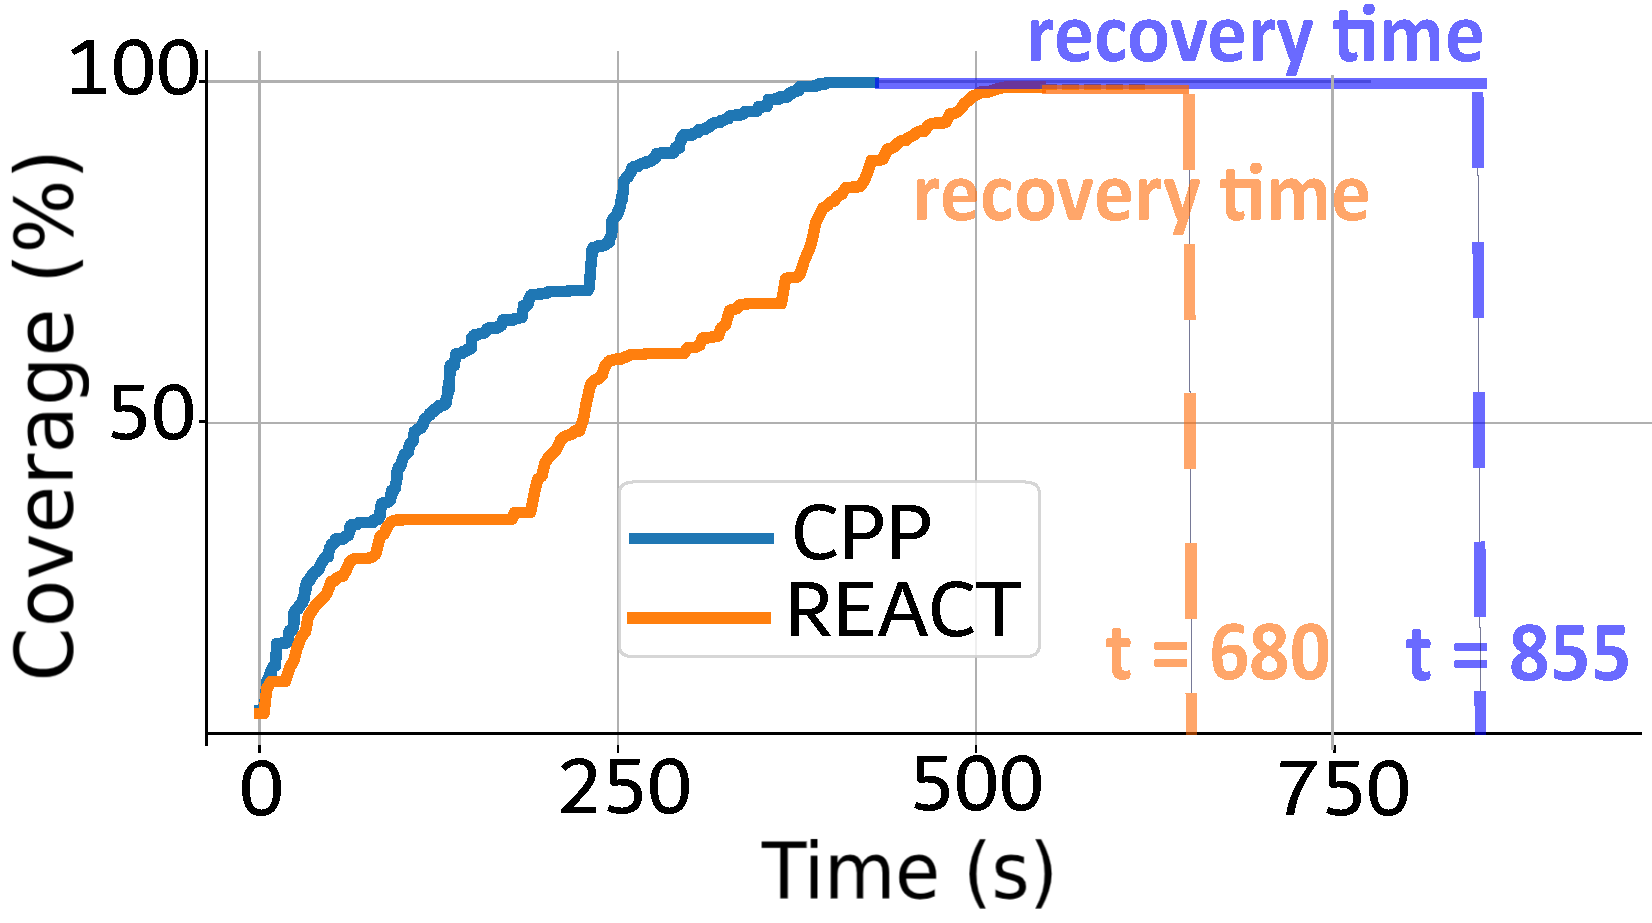
\includegraphics[width=\linewidth]
        {coverage_vs_time_recovery.pdf}
        %{coverage_vs_time.pdf}
        \caption{ Coverage vs. time.}
        \label{fig:coverage_vs_time}
    \end{subfigure}
    \hfill
    \begin{subfigure}[b]{0.48\linewidth}
        \centering
        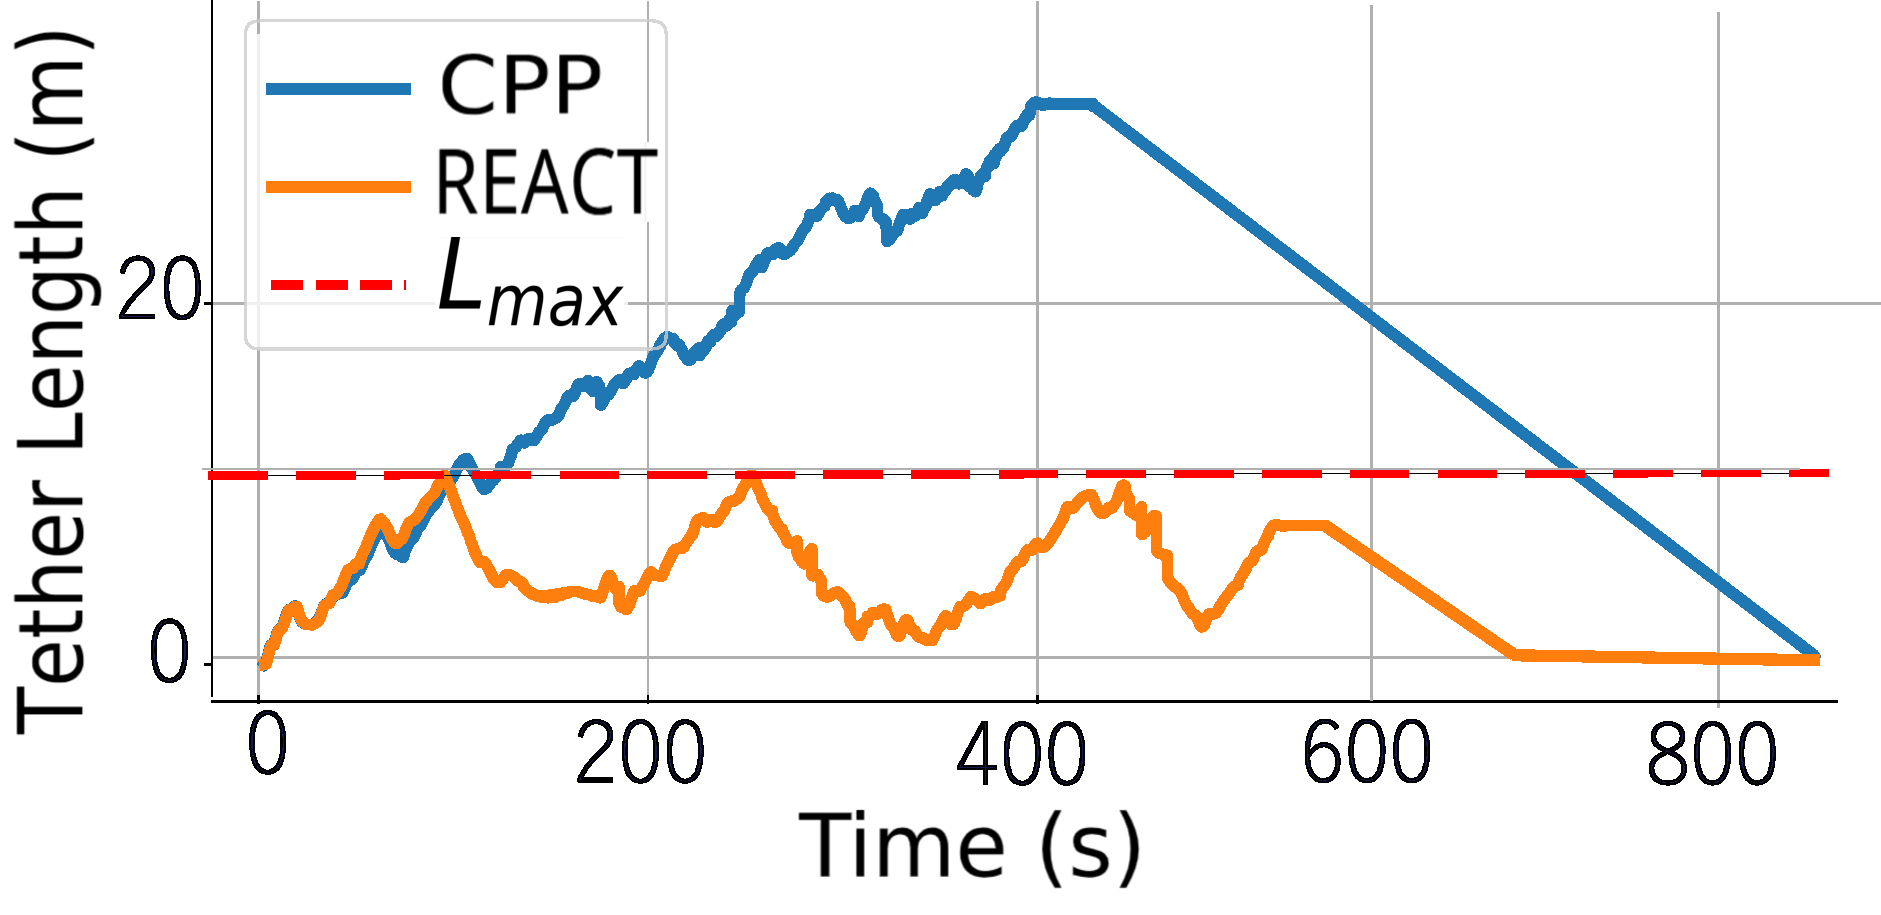
\includegraphics[width=\linewidth]{EA-Planner/figures/tether_length_vs_time_with_recovery.pdf}
        \caption{Tether Length vs. time.}
        \label{fig:tether_vs_time}
    \end{subfigure}
    \caption{Comparison of coverage and tether behavior over time.}
    \label{fig:coverage_tether_sidebyside}
\end{figure}


\begin{figure}[ht]
    \centering
    \begin{subfigure}[b]{0.48\linewidth}
        \centering
        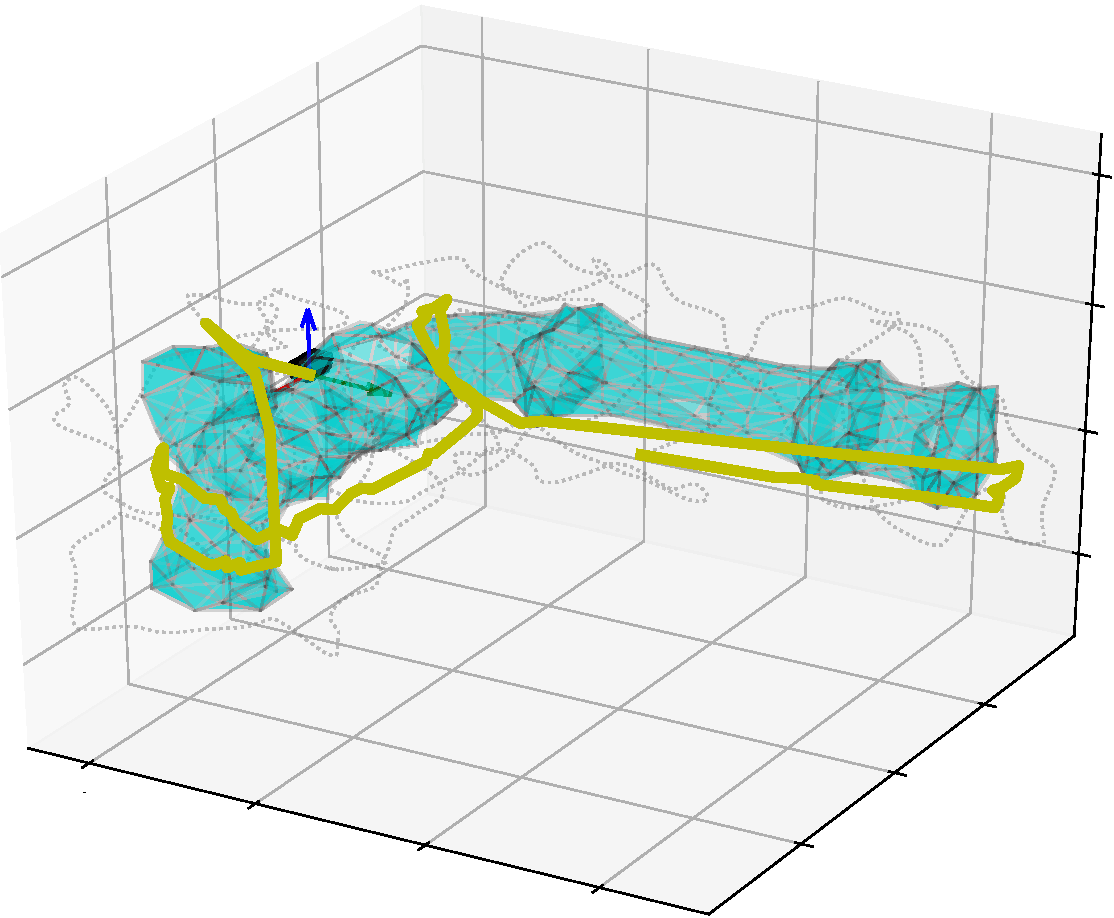
\includegraphics[width=\linewidth]{EA-Planner/figures/fc_planner_final_view.pdf}
        \caption{\ac{CPP} final tether path.}
        \label{fig:3d_cpp}
    \end{subfigure}
    \hfill
    \begin{subfigure}[b]{0.48\linewidth}
        \centering
        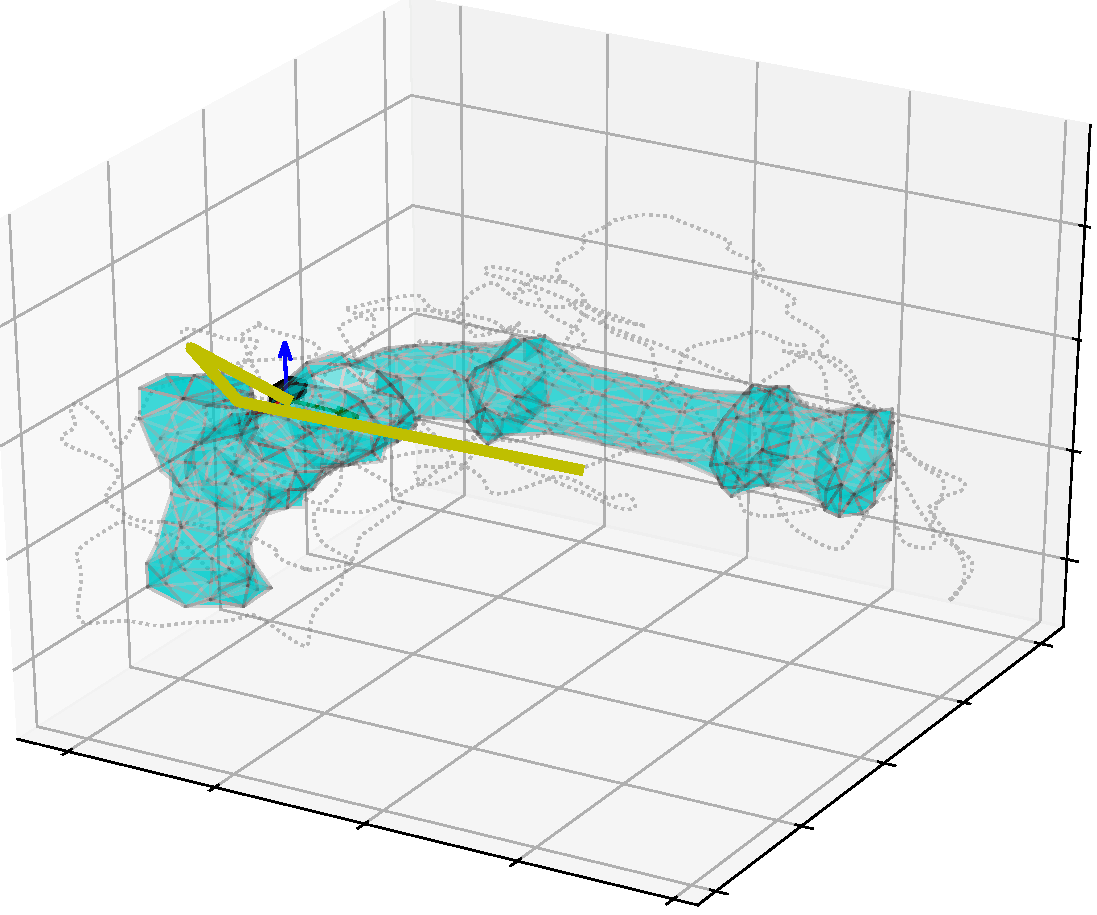
\includegraphics[width=\linewidth]{EA-Planner/figures/react_pipe.pdf}
        \caption{\ac{REACT} final tether path.}
        \label{fig:3d_oea}
    \end{subfigure}
    \caption{3D views of final trajectories. (a) CPP results in entangled tether path. (b) \ac{REACT} yields a non-entangled tether path, reflecting effective entanglement avoidance.}
    \label{fig:3Dplots}
\end{figure}
% The results highlight distinct trade-offs between the two planning strategies. The \ac{CPP}, lacking entanglement awareness, completed the trajectory significantly faster (429.00~s vs. 546.00~s) while achieving marginally less final coverage (99.81\% vs. 99.91\%). However, focusing solely on speed and final coverage overlooks the critical aspect of tether management in constrained environments. As shown in Figure~\ref{fig:tether_vs_time},\ac{CPP} planner exceeded the $L_{\text{max}}$ constraint during execution. 

% \ac{REACT} is explicitly designed to avoid and respond to potential tether entanglement. Its reactive replanning untangles the tether from entangled configurations. 

% Conversely, the \ac{CPP}, lacking entanglement- awareness, proceeds along its path violating the maximum tether length constraint. While this happened slightly later in this simulation, the approach risks encountering more severe or unrecoverable tether states without the ability to proactively mitigate them.

% The longer execution time of the \ac{REACT} directly is a result of executing reactive replanning maneuvers when necessary. This deliberate approach prioritizes tether safety and mission robustness over raw speed, offering a significant advantage for reliable operation in complex, real-world underwater scenarios where tether integrity is paramount. 

% The \ac{CPP}'s coverage speed advantage comes at the cost of ignoring potential tether hazards, making it less suitable for missions where entanglement poses a significant risk. Therefore, \ac{REACT} demonstrates superior performance in the context of safe and robust tethered \ac{ROV} operation, despite the longer completion time observed in this comparison.


The performance metrics for both planners are summarized in Table~\ref{tab:performance_metrics} and Table~\ref{tab:tether_metrics}, while Figures~\ref{fig:coverage_tether_sidebyside} and~\ref{fig:3Dplots} visualize the performance of the planners in terms of environmental coverage, tether length behavior, and final trajectory configurations. The evaluation focuses on comparing mission efficiency, constraint compliance, and safety aspects between the entanglement-aware \ac{REACT} method and the conventional \ac{CPP} baseline approach.



%The simulation experimental results demonstrate the effectiveness of our proposed \ac{REACT} method, which  continuously evaluates the tether path through the maximum tether length constraint. When \ac{REACT} detects potential entanglement or constraint violation, it dynamically finds alternative paths that disentangle the \ac{ROV} and then redirects toward the original waypoint. 

The results are presented in two phases: the inspection phase and the recovery phase, where the recovery time represents the estimated duration required to return to the starting position after complete inspection while disentangling the entire tether.

The results highlight distinct trade-offs between the two planning strategies. As shown in Table~\ref{tab:performance_metrics}, the \ac{CPP} method achieves a shorter inspection time (429s vs. 546s) due to its straightforward path execution without rerouting for disentanglement. However, focusing solely on inspection speed overlooks the critical aspect of tether management in constrained environments. The \ac{CPP} exhibits a significantly longer total mission time (855s vs. 680s) because extensive disentanglement is required after inspection completion.

The \ac{REACT} method demonstrates multiple instances of detection and resolution of entanglement, evidenced by the peaks in the tether length curve in Figure~\ref{fig:tether_vs_time} and the corresponding flat regions in the coverage curve in Figure~\ref{fig:coverage_vs_time}, where the \ac{ROV} inspection progress is stopped to reroute and find entanglement-free paths. This reactive replanning behavior directly results in the longer inspection time, as the system prioritizes tether safety over raw speed.

Notably, the tether length constraint is rarely exceeded by \ac{REACT} (maximum 10.52m vs. constraint of 10.0m), as shown in Table~\ref{tab:tether_metrics}. Conversely, the \ac{CPP} method severely violates this constraint, reaching 31.16m for extended periods (327.37s), risking unrecoverable tether states without the ability to proactively mitigate them. The 3D trajectory visualizations in Figure~\ref{fig:3Dplots} further illustrate this difference, showing the entangled tether geometry resulting from \ac{CPP} versus the non-entangled configuration achieved by \ac{REACT}. Therefore, \ac{REACT} demonstrates superior performance for safe tethered \ac{ROV} inspection.

 % 

\section{Conclusion & Future Work}
\label{sec:conclusion}
We presented \ac{REACT} a real-time entanglement-aware path planning framework for tethered \ac{ROV}'s operating in constrained underwater environments. Through comparative simulations, we demonstrated that while conventional planners may complete missions faster, they lack the ability to handle tether-related challenges effectively. \ac{REACT} mitigates potential entanglement through reactive replanning, offering a more robust and reliable solution. Despite a moderate increase in execution time, the entanglement-aware planner improves mission safety and integrity, making it a preferable choice for high-risk, cluttered inspection scenarios where tether management is critical. 

As future work, an experimental validation setup will be established to evaluate \ac{REACT} in a real-world test scenario. 



%Furture work will involve creating a ros plugin and integration with the UNav-sim simulator.


 % 0.25 page

%\appendix
%\section{Projection and Back-Projection}
%\input{sections/projection}

\section*{Acknowledgment}
This research receives support from Innovation Fund Denmark grant number 2040-00032B and EIVA a/s. The authors would also like to express their gratitude to Dr. Louis Petit from Université de Sherbrooke for his valuable insights on the ropeRRT path planner method and for open-sourcing his implementation using the OMPL library.
\bibliographystyle{IEEEtran}
% argument is your BibTeX string definitions and bibliography database(s)
\bibliography{References.bib}
%
% <OR> manually copy in the resultant .bbl file
% set second argument of \begin to the number of references
% (used to reserve space for the reference number labels box)

\end{document}
